\chapter{Results}\label{sec:results}


% shorten stress, computeState output is wrong. 
% Does it work and only the output is wrong or is the computation wrong? Yes is works only output is wrong. Now testing without output of computeStateInformation
% Output seems to fail only on lower ranks of every fiber. Now adding some debugging output.
% pcsgs02: fast_fibers_shorten_emg

% fibers_emg: 
% - use script to create MU distributions with mode 3
% - EMG signal of 3 single MUs (low location, high location, smaller, bigger) + final
% - same experiment fibers_emg vs. fibers_fat_emg -> see attenuation with spatial discrete fourier transform
% - same experiment with different mesh, numbers of fibers, scaling from small number up to a high number

% using electrodes: 
% - compare the two simulation results that were given to DEMUSE, this is a different scenario than fibers_emg

% todo:
% - fibers_emg vs. fibers_fat_emg    ~running
% - check mesh files, consolidate (needed for next point)  ~running
% - start highly resolved fibers_emg simulations on Hawk, with same mus
% - start precice coupling with shorten
% - add first experiments with validation, Hermite etc.

\section{Fiber Based Electrophysiology}
%\iffalse

In the following section, we simulate EMG signals on the upper arm. The simulation domain consists of the biceps brachii muscle, adipose tissue and the skin surface. We consider the multi-scale model of fiber based electrophysiology, where the monodomain equation \cref{eq:monodomain} is solved on several independent 1D muscle fibers. The membrane voltage $V_m$ is mapped from the 1D meshes to the 3D mesh. The static bidomain equation \cref{eq:bidomain1} is subsequently solved on the muscle and fat domains at fixed timesteps of the simulation.

\subsection{Effects of Single Motor Units on the Electromyography Signal}

The scenario contains 20 MUs that have an exponentially progressing number of fibers as shown in \cref{fig:MU_fibre_distribution_37x37_20c_txt_fiber_distribution}. The progression follows the function $y=1.1^x$.
The MU assignment is created using method 1a of the algorithm described in \cref{sec:muscle_fibers_and_motor_units}, where the MU territories are centered around given points and neighboring fibers are never part of the same MU. 

\Cref{fig:MU_fibre_distribution_37x37_20c_txt_2d_fiber_distribution} shows the fibers that are assigned to the smallest and largest MUs, MUs 1 and 20. For this visualization, the muscle cross-section is mapped to the large gray square and every colored small square corresponds to one fiber. The purple and red crosses designate the center of MU territories for MU 1 and 20, respectively. In consequence, the fibers of MU 1 are mostly located at the bottom left of the cross-section and the fibers of MU 20 are mostly located in the upper right regions of the muscle cross-section.
The visualization shows that the fibers of the same MU always have some spacing between them, which is due to the construction of the MU assignment algorithm.

% multidomain Vm
\begin{figure}[H]
  \centering%
  \begin{subfigure}[t]{\textwidth}%
    \centering%
    \includegraphics[width=0.6\textwidth]{images/results/application/MU_fibre_distribution_37x37_20c_txt_fiber_distribution_.pdf}%
    \caption{Exponential distribution of motor unit sizes. The abscissa axis shows the motor unit number, the ordinate axis shows their sizes or number of fibers belonging to each motor unit.}%
    \label{fig:MU_fibre_distribution_37x37_20c_txt_fiber_distribution}%
  \end{subfigure}\\
  \begin{subfigure}[t]{\textwidth}%
    \centering%
    \includegraphics[width=0.6\textwidth]{images/results/application/MU_fibre_distribution_37x37_20c_txt_2d_fiber_distribution_.pdf}%
    \caption{Fibers that belong to motor units 1 and 20.}%
    \label{fig:MU_fibre_distribution_37x37_20c_txt_2d_fiber_distribution}%
  \end{subfigure}
  \caption{Assignment of the 1369 fibers to 20 motor units used in the simulation scenario for fiber based electrophysiology.}%
  \label{fig:MU_fibre_distribution_37x37_20c}%
\end{figure}%

We begin with a simulation scenario where only a single MU is stimulated and study the effect on the surface EMG. The fibers of the respective MU are stimulated with a frequency $f=\SI{24}{\hertz}$ starting at time $t=\SI{0}{\milli\second}$. 
Each of the $13\times 13=\num{1369}$ fibers consists of a mesh with 1481 nodes, the 3D mesh of the muscle contains $19 \times 19 \times 38 = \num{13718}$ nodes and the 3D mesh of the fat layer contains $37 \times 5 \times 38 = \num{7030}$ nodes. The domains are partitioned to 27 processes. The subcellular model of Hodgkin and Huxley is used, yielding a total number of more than $\num{8.1e6}$ degrees of freedom. 
The timestep widths are $\dt_\text{0D}=\dt_\text{splitting} = \SI{2.5e-3}{\milli\second}$, $\dt_\text{1D} = \SI{6.25e-4}{\milli\second}$ and $\dt_\text{3D} = \SI{5e-1}{\milli\second}$, leading to 4 subcycles for the 1D model in each splitting step and 200 splitting steps per solution of the bidomain equation.

We compute the linear systems for the initial potential flow problem to estimate fiber directions in the 3D domain and for the bidomain equation, which is solved in every timestep  using a conjugate gradient solver. 
The program uses the \code{FastMonodomainSolver} class for the electrophysiology model. The Thomas algorithm solves the linear system of the diffusion problem. We use the \code{`vc`} optimization type and employ the scheme to only compute active fibers and the subcellular problems that are not in equilibrium.

The computation of a simulated time span with $t_\text{end}=\SI{100}{\milli\second}$  on an AMD EPYC 7742 64-core processor with \SI{2492}{\mega\hertz} base frequency and \SI{1.96}{\tera\byte} RAM takes approximately $\SI{100}{\second}$ in the scenario that activates only the smallest MU and $\SI{126}{\second}$ in the scenario that activates only the largest MU.

\Cref{fig:result_mu1} shows the result for the scenario of activating the smallest MU, MU 1. In \cref{fig:mu01a}, the surface is shown in the background and colored according to the extracellular potential $\phi_e$, which represents the EMG signal. The muscle volume is not shown, instead, the active parts of the respective fibers are displayed as tubes in the 3D domain. Their color visualizes the value of the transmembrane voltage $V_m$. In every of these small tube segments, the rising and declining shape of an action potential can be observed by the color progression from blue over orange to red for the rising part and back to blue for the declining part.

In this scenario, the fibers of MU 1 are stimulated three times within the first $\SI{100}{\milli\second}$ at $\SI{0}{\milli\second}$, $\SI{41.6}{\milli\second}$ and $\SI{83.3}{\milli\second}$.  The innervation zone contains the starting points for the propagating stimulus on every fiber. The scenario positions the neuromuscular junctions randomly within the central $\SI{10}{\percent}$ of every muscle fiber. The activated parts of the fibers visible in \cref{fig:mu01a} correspond to the propagated action potentials of the last two stimulations in this scenario.

By comparing the results in \cref{fig:mu01a} with the fiber distribution in \cref{fig:MU_fibre_distribution_37x37_20c_txt_2d_fiber_distribution}, it can be seen that fibers of MU 1 are located opposite of the muscle surface, which is at the upper side of the cross-sectional square diagram in \cref{fig:MU_fibre_distribution_37x37_20c_txt_2d_fiber_distribution}. The left side of the diagram in \cref{fig:MU_fibre_distribution_37x37_20c_txt_2d_fiber_distribution} corresponds to the lower part of the skin in \cref{fig:mu01a}. This part of the skin is closer to the activated fibers and, thus, the effect on the surface EMG is highest for this region.

\Cref{fig:mu01b} shows the skin surface as seen from the back in \cref{fig:mu01a}. The active region is located on the right-hand side in this image.
It can be seen that the active region on the skin surface, which results from fibers of the activated MU 1, only spans a small portion of the surface.

% Mu no. 1
\begin{figure}[H]
  \centering%
  \begin{subfigure}[t]{0.7\textwidth}%
    \centering%
    \includegraphics[width=\textwidth]{images/results/application/mu01a.png}%
    \caption{Membrane voltage $V_m$ at active parts of the fibers (foreground) and EMG signals $\phi_e$ on the skin surface (background).}%
    \label{fig:mu01a}%
  \end{subfigure} \,
  \begin{subfigure}[t]{0.25\textwidth}%
    \centering%
    \includegraphics[width=\textwidth]{images/results/application/mu01b.png}%
    \caption{Resulting surface EMG.}%
    \label{fig:mu01b}%
  \end{subfigure}   
  \caption{Simulation result at $t=\SI{99.5}{\milli\second}$ where only motor unit 1 is activated.}%
  \label{fig:result_mu1}%
\end{figure}%

% Mu no. 20
\begin{figure}[H]
  \centering%
  \begin{subfigure}[t]{0.7\textwidth}%
    \centering%
    \includegraphics[width=\textwidth]{images/results/application/mu20a.png}%
    \caption{Membrane voltage $V_m$ at active parts of the fibers (foreground) and EMG signals $\phi_e$ on the skin surface (background).}%
    \label{fig:mu20a}%
  \end{subfigure} \,
  \begin{subfigure}[t]{0.25\textwidth}%
    \centering%
    \includegraphics[width=\textwidth]{images/results/application/mu20b.png}%
    \caption{Resulting surface EMG.}%
    \label{fig:mu20b}%
  \end{subfigure}   
  \caption{Simulation result at $t=\SI{99.5}{\milli\second}$ where only motor unit 20 is activated, analogous to \cref{fig:result_mu1}.}%
  \label{fig:result_mu20}%
\end{figure}%

\Cref{fig:result_mu20} shows the analogous scenario that activates MU 20 instead of MU 1 is shown. \Cref{fig:mu20a} shows that, now, more fibers are activated as MU 20 is larger than MU 1. According to the MU layout in \cref{fig:MU_fibre_distribution_37x37_20c_txt_2d_fiber_distribution}, the active fibers are also located closer to the skin surface. This layout results in a stronger EMG signal compared to the previous scenario. 

The color coding in the two scenarios in \cref{fig:result_mu1,fig:result_mu20} is identical, and it can be seen that the absolute value of the extracellular potential $\phi_e$ is larger in the scenario of MU 20. For the scenario with MU 1 in \cref{fig:result_mu1}, the value range of the extracellular potential $\phi_e$ is $[\SI{-0.473}{\milli\volt}, \SI{0.204}{\milli\volt}]$. For the scenario with MU 20 in \cref{fig:result_mu20}, it is $[\SI{-0.834}{\milli\volt}, \SI{0.579}{\milli\volt}]$, which is more than double the range.

\Cref{fig:mu20b} shows the overall EMG signal on the skin surface for MU 20. Compared to the result of MU 1 in \cref{fig:mu01b}, nearly the inverse region is activated. It can, thus, be observed that the EMG signal is highly influenced by the location and size of the MUs. MUs with territories closer to the skin surface have a larger effect on the EMG signals than MUs that are located further away. As seen in \cref{fig:mu01b}, the influence of fibers completely vanishes for more than a certain distance. On the contrary, the effects of several close fibers add up such that large MUs located near the surface have the most impact on the resulting EMG signal.

% 0/27 : This is opendihu 1.2, built Apr  2 2021, C++ 201402, GCC 10.2.0, current time: 2021/4/2 22:05:20, hostname: ipvs-epyc2, n ranks: 27
% 0/27 : Open MPI v3.1.6, package: Open MPI maierbn@ipvs-epyc1 Distribution, ident: 3.1.6, repo rev: v3.1.6, Mar 18, 2020
% 0/27 : File "/data/scratch/sgs/maierbn/opendihu/examples/electrophysiology/fibers/fibers_fat_emg/settings_fibers_fat_emg.py" loaded.
% 0/27 : ---------------------------------------- begin python output ----------------------------------------
% Loading variables from "20mus_activate_one_mu.py".                                             
% MU 0                                                                                           
%   radius: 40.0                                                                                 
%   cm: 0.58                                                                                     
%   activation_start_time: 10000                                                                 
%   stimulation_frequency: 24                                                                    
% MU 4                                                                                           
%   radius: 42.7067691737                                                                        
%   cm: 0.58                                                                                     
%   activation_start_time: 10000                                                                 
%   stimulation_frequency: 24                                                                    
% MU 8                                                                                           
%   radius: 45.63666317700952                                                                    
%   cm: 0.58                                                                                     
%   activation_start_time: 10000                                                                 
%   stimulation_frequency: 24                                                                    
% MU 12                                                                                          
%   radius: 48.80807467158288
%   cm: 0.58                                     
%   activation_start_time: 10000
%   stimulation_frequency: 24
% MU 16                                          
%   radius: 52.24091246590275
%   cm: 1.0                                      
%   activation_start_time: 10000
%   stimulation_frequency: 24
% scenario_name: 20mus_activate_only_mu_20,  n_subdomains: 3 1 9,  n_ranks: 27,  end_time: 100.0
% dt_0D:           2.5e-03, diffusion_solver_type:      cg
% dt_1D:           6.3e-04, potential_flow_solver_type: gmres
% dt_splitting:    2.5e-03, emg_solver_type:            cg, emg_initial_guess_nonzero: False
% dt_3D:           5.0e-01, paraview_output: True 
% output_timestep: 1.0e+00  stimulation_frequency: 0.1 1/ms = 100.0 Hz
% fast_monodomain_solver_optimizations: True, use_vc: True
% fiber_file:              /data/scratch/sgs/maierbn/opendihu/examples/electrophysiology/input/left_biceps_brachii_37x37fibers.bin
% fat_mesh_file:           /data/scratch/sgs/maierbn/opendihu/examples/electrophysiology/input/left_biceps_brachii_37x37fibers.bin_fat.bin
% cellml_file:             ../../../input/hodgkin_huxley_1952.c
% fiber_distribution_file: fiber_distribution/MU_fibre_distribution_37x37_20c.txt
% firing_times_file:       /data/scratch/sgs/maierbn/opendihu/examples/electrophysiology/input/MU_firing_times_always.txt
% ********************************************************************************
% prefactor: sigma_eff/(Am*Cm) = 0.0132 = 3.828 / (500.0*0.58)
% n fibers:              1369 (37 x 37), sampled by stride 2 x 2
% n points per fiber:    1481, sampled by stride 40
% 27 ranks, partitioning: x3 x y1 x z9                                                           
% 37 x 37 = 1369 fibers, per partition: 12 x 36 = 432                                            
% per fiber: 1D mesh    nodes global: 1481, local: 200                                                                                                                                          
%   sampling 3D mesh with stride 2 x 2 x 40                                                                                                                                                     
%     linear 3D mesh    nodes global: 19 x 19 x 38 = 13718, local: 6 x 19 x 5 = 570                                                                                                             
%     linear 3D mesh elements global: 18 x 18 x 37 = 11988, local: 6 x 18 x 5 = 540                                                                                                             
% number of degrees of freedom:                                                                  
%                     1D fiber:       1481  (per process: 200)                                   
%             0D-1D monodomain:       5924  (per process: 800)                                   
%  all fibers 0D-1D monodomain:    8109956  (per process: 345600)                                
%                  3D bidomain:      13718  (per process: 570)                                   
%                        total:    8123674  (per process: 346170)                                
%     fat mesh, n points total:    7030 (37 x 5 x 38), (per process: 6 x 5 x 5 = 150)            
% Debugging output about fiber firing: Taking input from file "/data/scratch/sgs/maierbn/opendihu/examples/electrophysiology/input/MU_firing_times_always.txt"
% First stimulation times                                      

\subsection{Effects of the Fat Layer on the Electromyography Signal}

% different fat meshes
\begin{figure}[H]
  \centering%
  \begin{subfigure}[t]{0.3\textwidth}%
    \centering%
    \includegraphics[width=\textwidth]{images/results/application/fibers_emg_mesh_no_fat.png}%
    \caption{Muscle mesh without fat layer.}%
    \label{fig:fibers_emg_mesh_no_fat}%
  \end{subfigure} \quad
  \begin{subfigure}[t]{0.3\textwidth}%
    \centering%
    \includegraphics[width=\textwidth]{images/results/application/fibers_emg_mesh_thin_fat.png}%
    \caption{Muscle with thin fat layer.}%
    \label{fig:fibers_emg_mesh_thin_fat}%
  \end{subfigure}  \quad
  \begin{subfigure}[t]{0.3\textwidth}%
    \centering%
    \includegraphics[width=\textwidth]{images/results/application/fibers_emg_mesh_thick_fat.png}%
    \caption{Muscle with thick fat layer.}%
    \label{fig:fibers_emg_mesh_thick_fat}%
  \end{subfigure}   
  \caption{Meshes for the muscle domains (blue) and the layer of adipose tissue (red) used in the study to compare different fat layer widths.}%
  \label{fig:fibers_emg_mesh_fat}%
\end{figure}%

In the next study, we investigate the effect of the fat layer on the resulting EMG signals. The same scenario as in the previous section is used, except that the size of the body fat domain is varied and the activated MUs are chosen differently. We consider the domains and meshes shown in \cref{fig:fibers_emg_mesh_fat}: Scenario (a) only considers the muscle domain without additional  fat layer. Scenario (b) adds a thin fat layer with thickness of $\SI{2}{\milli\meter}$, discretized by two layers of finite elements. Scenario (c) considers a fat layer with thickness of $\SI{1}{\centi\meter}$ and four layers of elements. The scenario in the previous section also used this thick fat layer.

In this series of experiments, the first 10 MUs are activated with different stimulation frequencies ranging from \SI{7}{\hertz} for the smallest MU to \SI{15.15}{\hertz} for MU 10. The runtime of the simulation for one scenario on the same hardware as in the previous section is approximately $\SI{9}{\minute}$.

\Cref{fig:fibers_emg_fat} shows the simulation results at $t=\SI{100}{\milli\second}$ for the three scenarios with different fat layers. The figure uses the same color coding for the extracellular potential $\phi_e$ in all three scenarios. It can be seen that the volume conduction in the fat layer significantly smooths the resulting EMG signal, especially for the thick fat layer. The scenarios with no fat layer and a thin fat layer also exhibit a small difference.
This effect has implications for experimental studies, where the EMG recordings capture the less resolved spatial information, the more tissue is located between the muscle and the surface electrodes.

% results for different fat meshes
\begin{figure}[H]
  \centering%
  \begin{subfigure}[t]{0.36\textwidth}%
    \centering%
    \includegraphics[width=\textwidth]{images/results/application/fibers_emg_no_fat.png}%
    \caption{Simulation without fat layer.}%
    \label{fig:fibers_emg_no_fat}%
  \end{subfigure} \quad
  \begin{subfigure}[t]{0.25\textwidth}%
    \centering%
    \includegraphics[width=\textwidth]{images/results/application/fibers_emg_thin_fat.png}%
    \caption{Simulation with a thin fat layer.}%
    \label{fig:fibers_emg_thin_fat}%
  \end{subfigure}  \quad
  \begin{subfigure}[t]{0.28\textwidth}%
    \centering%
    \includegraphics[width=\textwidth]{images/results/application/fibers_emg_thick_fat.png}%
    \caption{Simulation with a thick fat layer.}%
    \label{fig:fibers_emg_thick_fat}%
  \end{subfigure}   
  \caption{Simulated surface EMG signals for the different fat layers shown in \cref{fig:fibers_emg_mesh_fat}.}%
  \label{fig:fibers_emg_fat}%
\end{figure}%

\begin{reproduce}
  The simulations in this section use the examples \code{examples/electrophysiology/fibers/fibers_emg} and \code{examples/electrophysiology/fibers/fibers_fat_emg} with the variables file \code{20mus_fat_comparison.py}.

  The scenario data that is necessary to run the simulations in \cref{a} are given in the repository at \href{https://github.com/dihu-stuttgart/performance}{github.com/dihu-stuttgart/performance}
  in the directory \code{opendihu/18_fibers_emg}. The main scripts that runs the simulations for the two sections are the following:
  \begin{lstlisting}[columns=fullflexible,breaklines=true,postbreak=\mbox{\textcolor{gray}{$\hookrightarrow$}\space}]
    ./run_single_MUs.sh
    ./run_compare_fat_layer.sh
  \end{lstlisting}
\end{reproduce}

\subsection{Effects of the Mesh Width on the Electromyography Signal}\label{sec:effects_of_the_mesh_width_emg}

Next, the simulated EMG signal is compared for different numbers of fibers and 3D mesh widths. We consider a scenario with 100 MUs and scale up the spatial resolution and the number of processes for the computation on the supercomputer Hawk at the High Performance Computing Center Stuttgart.

% fibers mesh
\begin{figure}[H]
  \centering%
  \includegraphics[width=0.5\textwidth]{images/results/application/MU_fibre_distribution_523x523_100mus_txt_mu_positions.pdf}%
  \caption{MU territory center points. The shown center points of the 100 motor units are used in all scenarios of the study with different numbers of fibers.}%
  \label{fig:MU_fibre_distribution_523x523_100mus_txt_mu_positions}%
\end{figure}

We compute scenarios with between \num{1369} and \num{76729} fibers. The 100 MUs have to be accordingly assigned to these numbers of fibers.
We use the method 1a of the algorithm described in \cref{sec:muscle_fibers_and_motor_units}. The MU territories are centered around pseudo-randomly generated center points, as shown in \cref{fig:MU_fibre_distribution_523x523_100mus_txt_mu_positions}. It can be seen that the MU territory center points are homogeneously distributed in space.


% MU distributions
\begin{figure}
  \centering%
  \begin{subfigure}[t]{0.45\textwidth}%
    \centering%
    \includegraphics[width=\textwidth]{images/results/application/MU_fibre_distribution_13x13_100mus_txt_fiber_distribution.pdf}%
    \caption{Size distribution for $13\times 13 = 169$ fibers.}%
    \label{fig:mus_13}%
  \end{subfigure} \quad
  \begin{subfigure}[t]{0.45\textwidth}%
    \centering%
    \includegraphics[width=\textwidth]{images/results/application/MU_fibre_distribution_37x37_100mus_txt_fiber_distribution.pdf}%
    \caption{Size distribution for $37\times 37 = 1369$ fibers.}%
    \label{fig:mus_37}%
  \end{subfigure}  \\
  \begin{subfigure}[t]{0.45\textwidth}%
    \centering%
    \includegraphics[width=\textwidth]{images/results/application/MU_fibre_distribution_187x187_100mus_txt_fiber_distribution.pdf}%
    \caption{Size distribution for $187\times 187 = \num{34969}$ fibers.}%
    \label{fig:mus_187}%
  \end{subfigure} 
  \begin{subfigure}[t]{0.45\textwidth}%
    \centering%
    \includegraphics[width=\textwidth]{images/results/application/MU_fibre_distribution_523x523_100mus_txt_fiber_distribution.pdf}%
    \caption{Size distribution for $523\times 523 = \num{273529}$ fibers.}%
    \label{fig:mus_523}%
  \end{subfigure}   
  \caption{Distribution of the sizes of the 100 MUs for the scenarios with different number of fibers.}%
  \label{fig:mu_sizes_100mus}%
\end{figure}%


For every fiber, the algorithm assigns a MU with a close center point with higher probability than a MU whose center is located further away. The total number of fibers per MU is progressing exponentially for the MUs from 1 to 100. The progression is described by an exponential function with basis $1.02$. \Cref{fig:mu_sizes_100mus} shows the MU size distributions for four scenarios with an increasing number of fibers from \num{169} to \num{273529}. For 169 fibers in \cref{fig:mus_13}, not all 100 MUs get associated with a fiber. It can be further seen that the error of the actual size distribution to the exponential function decreases with increasing number of fibers. For the largest scenario in \cref{fig:mus_523} the MU sizes range from 602 to 6097 fibers.

The number of fibers in the largest scenario matches the realistic number in a biceps muscle. The number of MUs can be higher in reality, e.g., by a factor of 5. Thus, the MUs in this scenario can be seen as a combination of multiple real MUs. Especially the smallest MUs, which in reality can consist of only some dozens of fibers are lumped by the first few MUs in our scenario. We restrict the number of MUs to 100 to be able to simulate the same problem also with smaller resolutions such as with 169 fibers.

\begin{figure}
  \centering%
  \begin{subfigure}[t]{0.47\textwidth}%
    \centering%
    \includegraphics[width=\textwidth]{images/results/application/MU_fibre_distribution_523x523_100mus_txt_0_2d_fiber_distribution_.png}%
    \caption{Partial problem with a quarter of the whole set of fibers and 25 MUs, which occurs in the algorithm 1a described in \cref{sec:muscle_fibers_and_motor_units}. Only three MUs are shown. The MU territory centers are indicated by the crosses.}%
    \label{fig:mu_assignment_part0}%
  \end{subfigure} \quad
  \begin{subfigure}[t]{0.47\textwidth}%
    \centering%
    \includegraphics[width=\textwidth]{images/results/application/MU_fibre_distribution_523x523_100mus_txt_2d_fiber_distribution_.png}%
    \caption{The resulting assignments of Mus to fibers, only shown for six MUs.}%
    \label{fig:mu_assignment_total}%
  \end{subfigure} 
  \caption{Association of MUs to the fibers. The square domain corresponds to a cross-section in the muscle, every colored point is one fiber and the color corresponds to the MU. }%
  \label{fig:mu_assignment_100}%
\end{figure}%

As described in \cref{sec:muscle_fibers_and_motor_units}, the MU assignment algorithm asserts that neighboring fibers are never part of the same MU by splitting the assignment problem for the given set of fibers into four smaller problems and finally interleaving the results of the four parts. \Cref{fig:mu_assignment_part0} shows such a part, where 25 MUs are associated to a subset of the fibers for the largest scenario of \num{273529} fibers. It can be seen that the three visualized MUs are largely clustered around their MU territory centers.

The final association of fibers and MUs is given in \cref{fig:mu_assignment_total}. Six selected MUs are shown of which the first, MU 1, corresponds to the first MU in \cref{fig:mu_assignment_part0}. The figure visualizes that the fibers especially of the MUs are distributed far across the muscle in this scenario. The comparison of the smallest MU, MU 1, and the largest MU, MU 100, shows the difference in MU sizes.


\begin{table}
  \centering%
  \begin{tabular}{|r|c|c|c|r|r|c|c|}
    \hline
    \#fibers        & \multicolumn{2}{c|}{3D stride} & 2D surface  & 3D dofs    & 0D dofs & \#proc. & \#comp.\\
    \cline{2-3}
                  & $x,y$    & $z$                         & mesh   &      &  && nodes\\
    \hline
    $37^2=\num{1369}$          & 2     & 8 & $19 \times 186$  & \num{67146}     & \num{8109956}  & \num{144} & 3\\[2mm]  % 6x6x4
    $67^2=\num{4489}$          & 2     & 4 & $34 \times 371$  & \num{428876}     & \num{26592836}  & \num{448} & 7\\[2mm]  % 7x8x8
    $109^2=\num{11881}$          & 2     & 3 & $55 \times 495$  & \num{1497375}     & \num{70383044}  & \num{1152} & 18\\[2mm]  % 12x12x8
    $187^2=\num{34969}$          & 2     & 2 & $94 \times 741$  & \num{6547476}     & \num{207156356}  & \num{3600} & 57\\ % 15x15x16
    \hline
  \end{tabular}
  \caption{Parameters of spatial discretization and parallel partitioning for the EMG study. The 3D stride refers to the stride with which the 3D mesh is generated from the 0D points. The 2D surface is the output of the EMG and corresponds to one face of the 3D mesh.}%
  \label{tab:emg_study_parameters}%
\end{table}

The numeric parameters of the simulations are the same as in the last section. The scenario is computed for a simulation time span of $\SI{1}{\s}$. The MUs are activated in a ramp every $\SI{2}{\ms}$ such that all MUs are active after $\SI{200}{\ms}$. The fiber radius
and the stimulation frequency for the MUs are exponentially distributed with basis $1.02$, similar to the MU size. The fiber radius increases from \SI{40}{\micro\meter} to \SI{55}{\micro\meter} and the stimulation frequency decreases from \SI{24}{\hertz} to \SI{7}{\hertz} over the MUs. A random frequency jitter of \SI{10}{\percent} is assumed.

The surface to volume ratio $A_m$ of the membrane is determined by assuming a cylindrical shape and can be computed from the fiber radius $r$ by $A_m = 2/r$ \cite{Klotz2020}. We model \SI{70}{\percent} slow twitch and \SI{30}{\percent} fast twitch fibers. Accordingly, the membrane capacitance $C_m$ is set to $C_m = \SI{0.58}{\micro\farad\per\centi\meter\squared}$ for the 70 smallest MUs and to $C_m = \SI{1}{\micro\farad\per\centi\meter\squared}$ for the 30 largest MUs.

The spatial discretization and parallel partitioning parameters are listed in \cref{tab:emg_study_parameters}. The first column shows the number of fibers. Their number increases, however, the mesh resolution in every fiber stays constant at 1480 elements per fiber. The stride that defines the 3D mesh is given in the second and third columns. The stride in radial direction of the muscle, i.e., the $x$ and $y$ coordinate directions, stays constant. Because the fiber density increases, the 3D mesh is refined accordingly. The stride along the fibers, i.e., in $z$ direction is reduced such that the mesh widths of the 3D mesh in all three coordinate directions remain balanced.

The resulting EMG recording of each simulation is described by a 2D mesh, which contains the values of the 3D muscle mesh without fat layer on the surface at one side of the muscle. \Cref{tab:emg_study_parameters} lists the dimension of this surface mesh in the fourth column. 
The number of dofs in the 3D mesh and the number of dofs in all fibers are listed in the next two columns. For these scenarios, it is not practical to output the 3D mesh or the 1D fiber meshes in regular time intervals, because this would produce a large amount of data that can hardly be processed. Instead, we output only the 2D surface mesh in the ParaView format every \SI{10}{\milli\second}.
\Cref{tab:emg_study_parameters} lists the number of processes and compute nodes on Hawk in the last two columns.

\Cref{fig:emg_hpc} shows the resulting surface EMG for four different resolutions at $t=\SI{179.5}{\ms}$. The color visualizes the value of the extracellular potential $\phi_e$ according to the shown color bar. Because of sign conventions in the definitions of the electric potentials, the EMG signals that correspond to muscle activation are negative.

The resulting electric potentials in \cref{fig:emg_hpc} exhibit different regions of higher activation that move over time from the center of the muscle towards its ends. The size of these regions decreases from \cref{fig:emg37} to \cref{fig:emg187} as the mesh width decreases. 
Dark-colored strong signals are visible, which mainly correspond to fibers that are directly underneath the shown muscle surface.
Apart from these strong signals, also weaker artifacts occur, which are shown in yellow and orange colors. They result from the superposition of several fibers of the same or different MUs. The number of recognizable weak signals is higher for the simulations with higher numbers of fibers and finer mesh resolution.

% results for different mesh widths
\begin{figure}
  \centering%
  \begin{subfigure}[t]{0.19\textwidth}%
    \centering%
    \includegraphics[height=12cm]{images/results/application/emg37.png}%
    \caption{$1369$ fibers}%
    \label{fig:emg37}%
  \end{subfigure} \,
  \begin{subfigure}[t]{0.19\textwidth}%
    \centering%
    \includegraphics[height=12cm]{images/results/application/emg67.png}%
    \caption{$4489$ fibers}%
    \label{fig:emg67}%
  \end{subfigure}  \,
  \begin{subfigure}[t]{0.19\textwidth}%
    \centering%
    \includegraphics[height=12cm]{images/results/application/emg109.png}%
    \caption{$\num{11881}$ fibers}%
    \label{fig:emg109}%
  \end{subfigure}    \,
  \begin{subfigure}[t]{0.35\textwidth}%
    \centering%
    \includegraphics[height=12cm]{images/results/application/emg187.png}%
    \caption{$\num{34969}$ fibers}%
    \label{fig:emg187}%
  \end{subfigure}   
  \caption{Simulated surface EMG signals for different numbers of fibers and different mesh widths of the 3D mesh.}%
  \label{fig:emg_hpc}%
\end{figure}%

% single figure of the largest scenario, also with mesh width shown
% 2d fiber distribution for the largest scenario that was run

%partitioning  2* 2* 1=    4    7^2=    49 fibers, fibers/rank: 12.250000, need    1 nodes
%partitioning  3* 3* 2=   18   13^2=   169 fibers, fibers/rank: 9.388889, need    1 nodes
%partitioning  4* 4* 4=   64   25^2=   625 fibers, fibers/rank: 9.765625, need    1 nodes
%partitioning  6* 6* 4=  144   37^2=  1369 fibers, fibers/rank: 9.506944, need    3 nodes
%partitioning  7* 8* 8=  448   67^2=  4489 fibers, fibers/rank: 10.020089, need    7 nodes
%partitioning 12*12* 8= 1152  109^2= 11881 fibers, fibers/rank: 10.313368, need   18 nodes
%partitioning 15*15*16= 3600  187^2= 34969 fibers, fibers/rank: 9.713611, need   57 nodes
%partitioning 22*22*16= 7744  277^2= 76729 fibers, fibers/rank: 9.908187, need  121 nodes
%partitioning 24*24*32=18432  427^2=182329 fibers, fibers/rank: 9.891981, need  288 nodes
%partitioning 29*29*32=26912  523^2=273529 fibers, fibers/rank: 10.163830, need  421 nodes
%partitioning 40*40*32=51200  523^2=273529 fibers, fibers/rank: 5.342363, need  800 nodes

% still in queue: 22*22*16= 7744  277^2= 76729 fibers on 121 nodes
%                 40*40*32=51200  523^2=273529 fibers, fibers/rank: 5.342363, need  800 nodes
% chained:
%partitioning 24*24*32=18432  427^2=182329 fibers, fibers/rank: 9.891981, need  288 nodes
%partitioning 29*29*32=26912  523^2=273529 fibers, fibers/rank: 10.163830, need  421 nodes

%% ---------------------------- 187 ------------------------------------------
%scenario_name: hawk2_fibers_emg_187,  n_subdomains: 15 15 16,  n_ranks: 3600,  end_time: 1000.0
%dt_0D:           2.5e-03, diffusion_solver_type:      cg
%dt_1D:           6.3e-04, potential_flow_solver_type: gmres, approx. exp.: True
%dt_splitting:    2.5e-03, emg_solver_type:            cg, emg_initial_guess_nonzero: True
%dt_3D:           5.0e-01, paraview_output: True, optimization_type: vc (AoVS)
%output_timestep: 1.0e+00, surface: 1.0e+01, stimulation_frequency: 0.1 1/ms = 100.0 Hz
%                          fast_monodomain_solver_optimizations: True
%fiber_file:              /lustre/cray/ws9/2/ws/icbbnmai-opendihu1/opendihu-hawk-gnu/examples/electrophysiology/input/left_biceps_brachii_187x187fibers.bin
%cellml_file:             /lustre/cray/ws9/2/ws/icbbnmai-opendihu1/opendihu-hawk-gnu/examples/electrophysiology/input/hodgkin_huxley_1952.c
%fiber_distribution_file: /lustre/cray/ws9/2/ws/icbbnmai-opendihu1/performance/opendihu/19_hawk_fibers_emg/fiber_distribution/MU_fibre_distribution_187x187_100mus.txt
%firing_times_file:       /lustre/cray/ws9/2/ws/icbbnmai-opendihu1/opendihu-hawk-gnu/examples/electrophysiology/input/MU_firing_times_always.txt
%********************************************************************************
%prefactor: sigma_eff/(Am*Cm) = 0.0132 = 3.828 / (500.0*0.58)
%diffusion solver type: cg
%n fibers:              34969 (187 x 187), sampled by stride 2 x 2
%n points per fiber:    1481, sampled by stride 2
%3600 ranks, partitioning: x15 x y15 x z16
%187 x 187 = 34969 fibers, per partition: 12 x 12 = 144
%per fiber: 1D mesh    nodes global: 1481, local: 94
%  sampling 3D mesh with stride 2 x 2 x 2
%    linear 3D mesh    nodes global: 94 x 94 x 741 = 6547476, local: 7 x 7 x 47 = 2303
%    linear 3D mesh elements global: 93 x 93 x 740 = 6400260, local: 7 x 7 x 47 = 2303
%number of degrees of freedom:
%                    1D fiber:       1481  (per process: 94)
%            0D-1D monodomain:       5924  (per process: 376)
% all fibers 0D-1D monodomain:  207156356  (per process: 54144)
%                 3D bidomain:    6547476  (per process: 2303)
%                       total:  213703832  (per process: 56447)
%
%% ---------------------------- 109 ------------------------------------------
%scenario_name: hawk2_fibers_emg_109,  n_subdomains: 12 12 8,  n_ranks: 1152,  end_time: 1000.0
%dt_0D:           2.5e-03, diffusion_solver_type:      cg
%dt_1D:           6.3e-04, potential_flow_solver_type: gmres, approx. exp.: True
%dt_splitting:    2.5e-03, emg_solver_type:            cg, emg_initial_guess_nonzero: True
%dt_3D:           5.0e-01, paraview_output: True, optimization_type: vc (AoVS)
%output_timestep: 1.0e+00, surface: 1.0e+01, stimulation_frequency: 0.1 1/ms = 100.0 Hz
%                          fast_monodomain_solver_optimizations: True
%fiber_file:              /lustre/cray/ws9/2/ws/icbbnmai-opendihu1/opendihu-hawk-gnu/examples/electrophysiology/input/left_biceps_brachii_109x109fibers.bin
%cellml_file:             /lustre/cray/ws9/2/ws/icbbnmai-opendihu1/opendihu-hawk-gnu/examples/electrophysiology/input/hodgkin_huxley_1952.c
%fiber_distribution_file: /lustre/cray/ws9/2/ws/icbbnmai-opendihu1/performance/opendihu/19_hawk_fibers_emg/fiber_distribution/MU_fibre_distribution_109x109_100mus.txt
%firing_times_file:       /lustre/cray/ws9/2/ws/icbbnmai-opendihu1/opendihu-hawk-gnu/examples/electrophysiology/input/MU_firing_times_always.txt
%********************************************************************************
%prefactor: sigma_eff/(Am*Cm) = 0.0132 = 3.828 / (500.0*0.58)
%diffusion solver type: cg
%n fibers:              11881 (109 x 109), sampled by stride 2 x 2
%n points per fiber:    1481, sampled by stride 3
%1152 ranks, partitioning: x12 x y12 x z8
%109 x 109 = 11881 fibers, per partition: 8 x 8 = 64
%per fiber: 1D mesh    nodes global: 1481, local: 186
%  sampling 3D mesh with stride 2 x 2 x 3
%    linear 3D mesh    nodes global: 55 x 55 x 495 = 1497375, local: 5 x 5 x 62 = 1550
%    linear 3D mesh elements global: 54 x 54 x 494 = 1440504, local: 5 x 5 x 62 = 1550
%number of degrees of freedom:
%                    1D fiber:       1481  (per process: 186)
%            0D-1D monodomain:       5924  (per process: 744)
% all fibers 0D-1D monodomain:   70383044  (per process: 47616)
%                 3D bidomain:    1497375  (per process: 1550)
%                       total:   71880419  (per process: 49166)
%
%% ---------------------------- 67 ------------------------------------------
%scenario_name: hawk2_fibers_emg_67,  n_subdomains: 7 8 8,  n_ranks: 448,  end_time: 1000.0
%dt_0D:           2.5e-03, diffusion_solver_type:      cg
%dt_1D:           6.3e-04, potential_flow_solver_type: gmres, approx. exp.: True
%dt_splitting:    2.5e-03, emg_solver_type:            cg, emg_initial_guess_nonzero: True
%dt_3D:           5.0e-01, paraview_output: True, optimization_type: vc (AoVS)
%output_timestep: 1.0e+00, surface: 1.0e+01, stimulation_frequency: 0.1 1/ms = 100.0 Hz
%                          fast_monodomain_solver_optimizations: True
%fiber_file:              /lustre/cray/ws9/2/ws/icbbnmai-opendihu1/opendihu-hawk-gnu/examples/electrophysiology/input/left_biceps_brachii_67x67fibers.bin
%cellml_file:             /lustre/cray/ws9/2/ws/icbbnmai-opendihu1/opendihu-hawk-gnu/examples/electrophysiology/input/hodgkin_huxley_1952.c
%fiber_distribution_file: /lustre/cray/ws9/2/ws/icbbnmai-opendihu1/performance/opendihu/19_hawk_fibers_emg/fiber_distribution/MU_fibre_distribution_67x67_100mus.txt
%firing_times_file:       /lustre/cray/ws9/2/ws/icbbnmai-opendihu1/opendihu-hawk-gnu/examples/electrophysiology/input/MU_firing_times_always.txt
%********************************************************************************
%prefactor: sigma_eff/(Am*Cm) = 0.0132 = 3.828 / (500.0*0.58)
%diffusion solver type: cg
%n fibers:              4489 (67 x 67), sampled by stride 2 x 2
%n points per fiber:    1481, sampled by stride 4
%448 ranks, partitioning: x7 x y8 x z8
%67 x 67 = 4489 fibers, per partition: 8 x 8 = 64
%per fiber: 1D mesh    nodes global: 1481, local: 188
%  sampling 3D mesh with stride 2 x 2 x 4
%    linear 3D mesh    nodes global: 34 x 34 x 371 = 428876, local: 5 x 5 x 47 = 1175
%    linear 3D mesh elements global: 33 x 33 x 370 = 402930, local: 5 x 5 x 47 = 1175
%number of degrees of freedom:
%                    1D fiber:       1481  (per process: 188)
%            0D-1D monodomain:       5924  (per process: 752)
% all fibers 0D-1D monodomain:   26592836  (per process: 48128)
%                 3D bidomain:     428876  (per process: 1175)
%                       total:   27021712  (per process: 49303)
%                       
%% ---------------------------- 37 ------------------------------------------
%scenario_name: hawk2_fibers_emg_37,  n_subdomains: 6 6 4,  n_ranks: 144,  end_time: 1000.0
%dt_0D:           2.5e-03, diffusion_solver_type:      cg
%dt_1D:           6.3e-04, potential_flow_solver_type: gmres, approx. exp.: True
%dt_splitting:    2.5e-03, emg_solver_type:            cg, emg_initial_guess_nonzero: True
%dt_3D:           5.0e-01, paraview_output: True, optimization_type: vc (AoVS)
%output_timestep: 1.0e+00, surface: 1.0e+01, stimulation_frequency: 0.1 1/ms = 100.0 Hz
%                          fast_monodomain_solver_optimizations: True
%fiber_file:              /lustre/cray/ws9/2/ws/icbbnmai-opendihu1/opendihu-hawk-gnu/examples/electrophysiology/input/left_biceps_brachii_37x37fibers.bin
%cellml_file:             /lustre/cray/ws9/2/ws/icbbnmai-opendihu1/opendihu-hawk-gnu/examples/electrophysiology/input/hodgkin_huxley_1952.c
%fiber_distribution_file: /lustre/cray/ws9/2/ws/icbbnmai-opendihu1/performance/opendihu/19_hawk_fibers_emg/fiber_distribution/MU_fibre_distribution_37x37_100mus.txt
%firing_times_file:       /lustre/cray/ws9/2/ws/icbbnmai-opendihu1/opendihu-hawk-gnu/examples/electrophysiology/input/MU_firing_times_always.txt
%********************************************************************************
%prefactor: sigma_eff/(Am*Cm) = 0.0132 = 3.828 / (500.0*0.58)
%diffusion solver type: cg
%n fibers:              1369 (37 x 37), sampled by stride 2 x 2
%n points per fiber:    1481, sampled by stride 8
%144 ranks, partitioning: x6 x y6 x z4
%37 x 37 = 1369 fibers, per partition: 6 x 6 = 36
%per fiber: 1D mesh    nodes global: 1481, local: 376
%  sampling 3D mesh with stride 2 x 2 x 8
%    linear 3D mesh    nodes global: 19 x 19 x 186 = 67146, local: 3 x 3 x 47 = 423
%    linear 3D mesh elements global: 18 x 18 x 185 = 59940, local: 3 x 3 x 47 = 423
%number of degrees of freedom:
%                    1D fiber:       1481  (per process: 376)
%            0D-1D monodomain:       5924  (per process: 1504)
% all fibers 0D-1D monodomain:    8109956  (per process: 54144)
%                 3D bidomain:      67146  (per process: 423)
%                       total:    8177102  (per process: 54567)
%

\begin{reproduce}
  Use the following commands to run the EMG simulation of the biceps muscle with fat layer and electrodes:
  \begin{lstlisting}[columns=fullflexible,breaklines=true,postbreak=\mbox{\textcolor{gray}{$\hookrightarrow$}\space}]
    cd $\$$OPENDIHU_HOME/examples/electrophysiology/fibers/fibers_fat_emg/build_release
    mpirun -n 16 fibers_fat_emg ../settings_fibers_fat_emg.py 50mus.py
    cd out/50mus
    plot_emg.py ./electrodes.csv ./stimulation.log 25900 26000    # plot the result, here for time span 25.9s - 26s
  \end{lstlisting}
\end{reproduce}


\subsection{Simulation of EMG electrodes}
% fibers_fat_emg with electrodes

While the surface EMG simulation results as presented in the last section in \cref{fig:emg_hpc} are suited for insights into the temporal and spatial variation of the electric potential, real experiments are constraint to capture values at the discrete locations of electrodes.
For some applications, such as the evaluation of EMG decomposition algorithms, it is beneficial to obtain simulated values at electrode locations.

One possibility would be to extract nodal values from the simulated surface meshes to simulate electrodes. However, the distance between the nodes in the mesh is not constant in the whole mesh, whereas EMG electrode arrays have a fixed inter electrode spacing. We, therefore, follow a different approach and allow to directly specify a grid of electrodes close to the muscle surface. These points are then mapped onto the surface of the muscle and the respective values are calculated by evaluating the finite element interpolant at the respective locations.

In OpenDiHu, a 2D grid of surface electrodes can be defined in the Python settings file by specifying the grid parameters and inter electrode distances. In result, the simulation distributes the electrodes to the processes according to the parallel partitioning of the 3D mesh, evaluates the computed EMG values at the respective locations and outputs them in a single text file of comma separated values.

\Cref{fig:fibers_fat_emg2_electrodes} shows a simulation of fiber based electrophysiology with 49 fibers, fat layer and an array of $12\times 32$ electrodes, which are visualized as spheres. The muscle fibers below the fat layer are colored according to the transmembrane voltage $V_m$. Only the surface of the fat layer is shown and colored according to the extracellular potential $\phi_e$. The electrodes take the same values as $\phi_e$ but are colored with the different \emph{EMG} color scale to make the resulting signal more distinguishable. Two activated bands across the muscle surface can be seen, which are also present in the electrode values.

\begin{figure}
  \centering%
  \includegraphics[width=0.7\textwidth]{images/results/application/fibers_fat_emg2.png}%
  \caption{Simulation of surface EMG and capturing electrodes. The scenario contains 49 muscle fibers, a fat layer of which only the surface is shown and a grid of $12 \times 32$ equidistant electrodes.}%
  \label{fig:fibers_fat_emg2_electrodes}%
\end{figure}

To visually evaluate the simulated EMG signals at the electrodes, OpenDiHu provides utility to create the visualizations shown in \cref{fig:emg_video}. \Cref{fig:emg_video_37} shows a still image from an animation. On the upper right, the grid of electrodes is displayed, the EMG signal is given by the color coding and changes over time. At the bottom of the image, the activation times of the MUs are visualized. Every horizontal line corresponds to one MU. The colored markers indicate, when the respective MU fires. As the shown example visualizes data for \SI{40}{\s}, the individual firing times are not visible. A vertical bar moves over the time axis and indicates the current time of the animation. The picture displays the EMG values at time $t=\SI{25.975}{\s}$. The upper right of the image shows a text with static information about the dataset, containing the electrode grid size, the inter electrode distance (IED), the end time, the sampling frequency of the electrodes, i.e., the frequency with which values are stored, and the number of MUs.

\Cref{fig:emg_video_plot} shows another, static visualization of simulated EMG data. The diagram contains tiles for every electrode in the $12\times 32$ grid. The value of the EMG signal is plotted over time for every electrode. The figure shows the data of \cref{fig:emg_video_37} for the time interval $[\SI{25.9}{\s},\SI{26}{\s}]$.
This visualization enables to visually identify propagating action potentials from the columns of tiles. The propagation velocity of the action potentials can be estimated from the time shift of matching spikes.

\begin{figure}
  \centering%
  \begin{subfigure}[t]{0.6\textwidth}%
    \centering%
    \includegraphics[width=\textwidth]{images/results/application/emg_video_37.png}%
    \caption{fibers mesh}%
    \label{fig:emg_video_37}%
  \end{subfigure}  \,
  \begin{subfigure}[t]{0.38\textwidth}%
    \centering%
    \includegraphics[width=\textwidth]{images/results/application/emg_video_plot.pdf}%
    \caption{Surface EMG at $12 \times 32$ electrodes in the time range $[\SI{25.9}{\s},\SI{26}{\s}]$.}%
    \label{fig:emg_video_plot}%
  \end{subfigure}
  \caption{Simulation of surface EMG using electrodes.}%
  \label{fig:emg_video}%
\end{figure}
%\fi
\subsection{Decomposition of Surface EMG Signals}

Surface EMG recordings are a valuable tool to gain insights into the neuromuscular system. They are used, e.g., for the diagnosis of muscular disorders and in clinical studies that aim to advance the biomedical understanding.

% why, how are EMG signals generated -> fig
The EMG signals on the skin surface originate from the activated muscle fibers. Effects from volume conduction of action potentials on all muscle fibers are superpositioned and contribute to the EMG signal according to their distance to the skin surface. As all fibers in the same MU get activated simultaneously, each MU's contribution shows a characteristic \say{shape} in the resulting surface EMG signal. This shape is influenced by the number and location of the muscle fibers relative to the electrodes and the location of the neuromuscular junctions.

In our simulation, the location of the neuromuscular junctions is chosen pseudo-randomly (but deterministic) during initialization in the central \SI{10}{\percent} of every muscle fiber. \Cref{fig:emg_video_37_junctions} shows the state of a simulation with $1369$ fibers at $t=\SI{1}{\ms}$, where all fibers were are activated at $t=\SI{0}{\ms}$. The color coding indicates the transmembrane potential $V_m$, which is only depolarized near the locations of the neuromuscular junctions.

\begin{figure}
  \centering%
  \includegraphics[width=0.7\textwidth]{images/results/application/emg_video_37_junctions.png}%
  \caption{Locations of the neuromuscular junctions}%
  \label{fig:emg_video_37_junctions}%
\end{figure}

% gCKC method
Methods exist that seek to decompose the surface EMG signal into the contributions of the individual MUs. One popular method is \emph{Gradient Convolution Kernel Compensation} (gCKC) \cite{Holobar2007b,Holobar2007}. 

Most decomposition methods, including the gCKC algorithm, assume that the EMG signal at an electrode is composed of the convolutional mixture of $N$ filters of the MU activity. 
The activity of each MU $k\in \{1,\dots,N\}$ is described by the innervation pulse trains that activate the fibers of MU $k$, i.e., neural inputs at stimulation times $\varphi_r$. The source signal $s_k$ in the muscle that represents the effect of MU $k$ is given as filter over these neural point processes, $s_k(t) = \sum_r\delta(t - \varphi_r)$, where $\delta$ is the dirac delta function.

The vector of observed EMG values $\bfx \in \R^m$ is composed of the temporal convolution over $L$ time-shifted sources $\bfs$ and a term $\bfomega$ of additive Gaussian noise:
\begin{align*}
  \bfx(t) = \s{l=0}{L-1}\bfH(l)\,\bfs(t-l) + \bfomega(t).
\end{align*}
Here, $\bfH$ is the $m\times n$ mixing matrix for $m$ observations and $n$ MU sources and $\bfs = (s_k)_{1,\dots,n}$ is the vector of source signals. The summation over $L$ previous values in this convolutive mixture can be reformulated by integrating it into the matrix-vector product. The dimensions of the matrix $\bfH$ and the vector $\bfs$ are extended accordingly. Inversion of the extended mixture matrix yields separation vectors, with which the innervation pulse trains of the MUs can be recovered from the recorded signals. The gCKC algorithm performs the inversion indirectly by solving a derived optimization problem with a gradient descent scheme.

The gCKC decomposition algorithm is available in the DEMUSE software, a commercial, MATLAB based tool that allows automatic and semi-automatic EMG decomposition \cite{demuse}. In collaboration with Lena Lehmann from the \emph{Institute of Signal Processing and System Theory} and the \emph{Institute for Modelling and Simulation of Biomechanical Systems}, we evaluated the performance of gCKC decomposition of simulated surface EMG signals.

% different performance depending on parameters
We simulate fiber-based electrophysiology scenarios with fat layer and 1369 fibers. The model parameter are the same as in \cref{sec:effects_of_the_mesh_width_emg}. In the first scenario, a fat layer with thickness of $\SI{1}{\cm}$ is used. The fibers are distributed to 20 MUs.
\Cref{emg_20mus-50s-old2} shows the firing times of the 20 MUs in the first \SI{10}{\second}. The MUs are initially activated every \SI{100}{\ms} to generate the shown \say{ramp} activation pattern, which later helps to identify the recovered MUs.  From $t=\SI{1.8}{\second}$ on, all MUs are firing with their own constant frequency, modified by a jitter of $\SI{10}{\percent}$.

The gCKC decomposition algorithm in the software DEMUSE was applied on the first $t=\SI{40}{\second}$ of simulated EMG data. The preconfigured algorithm was used without manual intervention.
While the simulated EMG recording consists of an electrode grid of $12 \times 32$ fibers, as shown in \cref{fig:emg_video}, only a rectangular subset of $5\times 13$ channels at the lower center of the grid was used for the decomposition to mimic a realistic electrode array size. The DEMUSE software discarded four of these 65 channels as being invalid.

\Cref{fig:emg_20mus-50s-old2} shows the innervation pulses that were detected by DEMUSE as red vertical markers. DEMUSE found four MUs in this scenario, i.e., \SI{20}{\percent}. 
The recovered MUs were identified in the set of simulated MUs by matching the activation onset time in the ramp scheme and the average firing frequency. A first visual comparison with the original stimulation times shows a good agreement.

The association of fibers with MUs follows an exponential MU size progression with a basis of approximately $1.2$, as shown in \cref{fig:oldmus_progression}. The smallest MU receives two fibers and the largest MU contains 256 fibers. The method 1 described in \cref{sec:method1_assignment} was used to generate the spatial association of fibers and MUs. \Cref{fig:oldmus_2d} depicts the location of the four MUs that were detected by DEMUSE. The detected MUs have the indices 16, 18, 19 and 20 and correspond to four of the five largest MUs. It can be seen that MUs 18 to 20 are located mainly in the upper half of the muscle cross-section, in proximity to the electrode array at the top of the diagram.
The MU with the most fibers, MU 20, was detected by the decomposition algorithm even though it is located at the lower left of diagram at a large distance to the skin surface.

% old
\begin{figure}
  \centering%
  \includegraphics[width=\textwidth]{images/results/application/emg_20mus-50s-old2.pdf}%
  \caption{a.}%
  \label{fig:emg_20mus-50s-old2}%
\end{figure}

Further scenario were simulated with the same parameters but 50 and 100 MUs. In these datasets, DEMUSE detected 8 and 12 MUs, which corresponds to \SI{16}{\percent} and \SI{12}{\percent}. Another scenario was computed with 20 MUs but a fat layer of only \SI{2}{\mm} instead of \SI{1}{\cm}. Moreover, the association scheme between MUs and fibers was changed as shown in \cref{fig:newmus}. The exponential distribution of MU sizes here only varied between 42 and 102 fibers per MU, corresponding to a basis in the exponential function of approximately $1.05$. 

\Cref{emg_20mus-40s_new} shows the results of the EMG decomposition with the gCKC algorithm. DEMUSE successfully decomposed the signal into 13 MUs corresponding to \SI{65}{\percent}. DEMUSE yielded two additional MUs, which we do not considered part of the set of successfully recovered MUs. The first only contains ten innervation pulses and the second pulse train consists of high frequency oscillations.
In this scenario, the software marked only one EMG recording channel as invalid, which means that more data was considered in the decomposition algorithm.

Similar to the previously presented scenario, the larger MUs are detected with a higher probability than the smaller MUs. In this scenario, the eight largest MUs are successfully found. \Cref{fig:newmus_2d} shows the spatial arrangement of the detected MUs. The parts of the muscle cross section that are occupied by undetected MUs is again more distance from the skin surface at the upper boundary. However, the recovered MUs 1 and 14 are located at the lower boundary, i.e., in the most distant area from the EMG electrodes. 

% new
\begin{figure}
  \centering%
  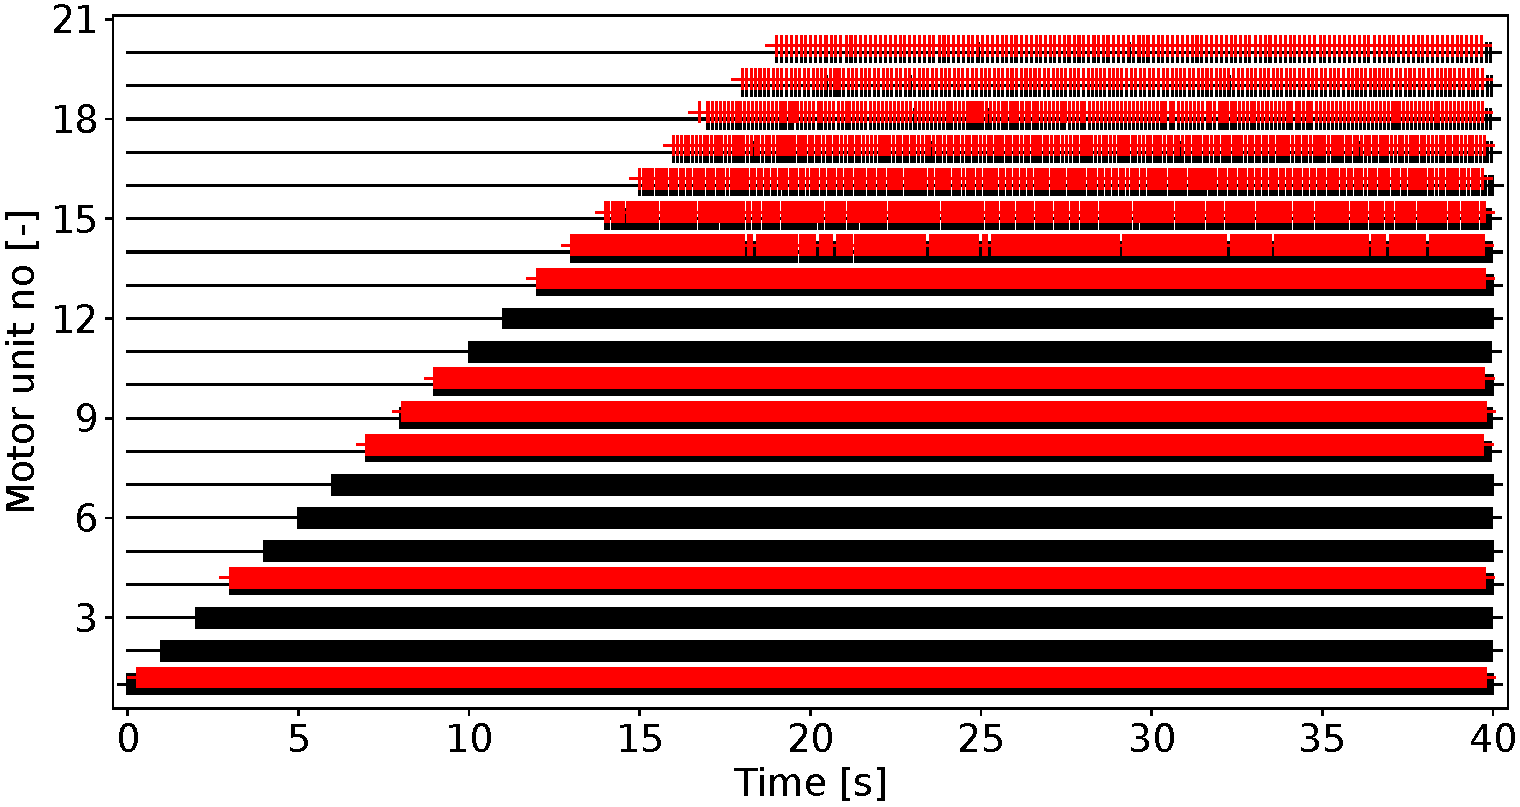
\includegraphics[width=\textwidth]{images/results/application/emg_20mus-40s_new3.pdf}%
  \caption{New}%
  \label{fig:emg_20mus-40s_new}%
\end{figure}

%-----

% old fiber distribution: Smallest MU: 2, Largest MU: 256
\begin{figure}
  \centering%  \,
  \begin{subfigure}[t]{0.45\textwidth}%
    \centering%
    \includegraphics[width=\textwidth]{images/results/application/oldmus2.pdf}%
    \caption{a.}%
    \label{fig:oldmus_progression}%
  \end{subfigure}\hfill
  \begin{subfigure}[t]{0.45\textwidth}%
    \centering%
    \includegraphics[width=\textwidth]{images/results/application/oldmus1.pdf}%
    \caption{a}%
    \label{fig:oldmus_2d}%
  \end{subfigure}
  \caption{Simulation of surface EMG using electrodes.}%
  \label{fig:oldmus}%
\end{figure}

% new fiber distribution: Smallest MU: 42, Largest MU: 102
% number fibers per MU: [ 50  45  43  51  43  42  50  53  61  71  72  69  78  97  87  87 102  74 101  93]
\begin{figure}
  \centering% \,
  \begin{subfigure}[t]{0.45\textwidth}%
    \centering%
    \includegraphics[width=\textwidth]{images/results/application/newmus1.pdf}%
    \caption{a.}%
    \label{fig:newmus_progression}%
  \end{subfigure}\hfill
  \begin{subfigure}[t]{0.45\textwidth}%
    \centering%
    \includegraphics[width=\textwidth]{images/results/application/newmus3.pdf}%
    \caption{a}%3
    \label{fig:newmus_2d}%
  \end{subfigure} 
  \caption{Simulation of surface EMG using electrodes.}%
  \label{fig:newmus}%
\end{figure}

\begin{figure}
  \centering%
  \begin{subfigure}[t]{0.47\textwidth}%
    \centering%
    \includegraphics[width=\textwidth]{images/results/application/emg_20mus-40s_new-noshift2.pdf}%
    \caption{a.}%
    \label{fig:newmus_nocorrection}%
  \end{subfigure}
  \caption{Simulation of surface EMG using electrodes.}%
  \label{fig:emg_video}\,
  \begin{subfigure}[t]{0.47\textwidth}%
    \centering%
    \includegraphics[width=\textwidth]{images/results/application/emg_20mus-40s_new-shift2.pdf}%
    \caption{a}%
    \label{fig:newmus_withcorrection}%
  \end{subfigure}
  \caption{Simulation of surface EMG using electrodes.}%
  \label{fig:newmus_shifting}%
\end{figure}

Next, we evaluate the quality of the innervation pulse trains that are recovered by the gCKC algorithm in our scenarios. We compare the stimulation times calculated by DEMUSE with the stimulation times of the simulation. \Cref{fig:newmus_nocorrection} shows an excerpt of the detected pulse trains of the scenario in \cref{fig:emg_20mus-40s_new}. We observe for some MUs that the recovered stimulation times are consistently shifted in time. This effect is especially visible for MUs 18 and 16. 

The  time points given by the simulation in OpenDiHu correspond to the times when the fibers are stimulated. The detected MU activation in DEMUSE, however, correspond to the time when the MU action potential shape in the EMG recording reaches its maximum.
Moreover, the exact time when a particular MU reaches a particular EMG electrode  depends on the distance of the electrode to the innervation points of the MU. The further the electrode is away from the neuromuscular junctions, the higher is the delay of the recorded spike to the corresponding innervation pulse. Thus, constant time shift in the pulses detected by the gCKC algorithm is valid and has to be accounted for in the evaluation.

We correct for this time shift by adding a constant time offset $\Delta t$ to the recovered innervation pulse trains. The algorithm finds the matching pairs of simulated and recovered pulses and optimizes the value of $\Delta t$ such that the time differences in these pairs after the shift correction get minimal.

\Cref{fig:newmus_withcorrection} shows the same extract of MU activity as in \cref{fig:newmus_nocorrection} with applied time offsets. The time offsets for MUs 14 to 18 are $\SI{-2.4}{\ms}, \SI{-1.1}{\ms}, \SI{-12.9}{\ms}, \SI{-2.9}{\ms}$ and $\SI{-24.9}{\ms}$. It can be seen that the recovered pulses now match the simulated data very well. The non-matching pulses are clearly false positive detections.

To compare the recovered MU times between the scenarios, we compute the rate of agreement metric. The MU firing times from the simulation serve as the ground truth to which we compare the recovered MU times. We identify true positive (TP), false positive (FP) and false negative (FN) recovered pulses, depending on whether a matching time can or cannot be found in the simulation data at that time within a tolerance of $\eps=\SI{5}{\ms}$. The rate of agreement (RoA) between the gCKC algorithm output and the ground truth data is then computed by%
\begin{align*}
  \textrm{RoA}  = \dfrac{\textrm{TP}}{\textrm{TP} + \textrm{FP} + \textrm{FN}}.
\end{align*}

In the first scenario in \cref{fig:emg_20mus-50s-old2}, the RoA for MUs 16,18 and 19 is above $\SI{99.7}{\percent}$ and only $\SI{82.2}{\percent}$ for MU 20. Only 296 of the 334 detected pulses are true positives, which corresponds to a precision of $\SI{88.6}{\percent}$.
% MU 16 from matlab: FP: 0, TP: 484, FN: 0 -> RoA: 1.0
% MU 18 from matlab: FP: 1, TP: 409, FN: 0 -> RoA: 0.9975609756097561
% MU 19 from matlab: FP: 1, TP: 370, FN: 0 -> RoA: 0.9973045822102425
% MU 20 from matlab: FP: 38, TP: 296, FN: 26 -> RoA: 0.822222222222222
 
In the other scenario presented in \cref{fig:emg_20mus-40s_new} all valid MUs except one have RoA values of above $\SI{94.5}{\percent}$. Five MUs are even detected perfectly with $\SI{100}{\percent}$ rate of agreement. MU 9 is the only detected MU with a degraded RoA of approximately $\SI{57.9}{\percent}$. However, the RoA improves to $\SI{98.1}{\percent}$, if the tolerance $\eps$ for matching pulses is relaxed to $\SI{10}{\ms}$. This shows that RoA metric also depends on a proper value for the tolerance $\eps$ and that the resulting innervation pulse trains of DEMUSE can have varying accuracy.
 
 %MU 9 from matlab: FP: 191, TP: 321, FN: 42 -> RoA: 0.5794223826714802
 
While the gCKC algorithm can be used for EMG decomposition of previously recorded signals in a controlled environment, it is less suited for real-time applications such as human-machine interfaces. The application of the trained separation vectors, which were obtained from the gCKC algorithm, on new data requires a certain history of previously captured data to calculate the decomposed MU pulses. This delays the predictions in HMI applications. Furthermore, the system is sensitive to noisy data. A fundamentally different approach to EMG decomposition is the use of sequence-to-sequence learning methods such as using recurrent neural networks. The authors of \cref{Clarke2021} used a gated recurrent unit (GRU) network for this task. The network was trained using the output of the gCKC algorithm and subsequently able to decompose surface EMG signals into innervation pulse trains. The approach was shown to also works for low signal-to-noise ratios.

To assess, whether our simulations of surface EMG can be used for the supervised learning of GRU networks for EMG decomposition, we tried to reproduce the studies of \cref{Clarke2021}, where the GRU is trained with the output of the gCKC algorithm. Additionally, we trained a GRU network directly on the simulated EMG data. These tasks were carried out in the masters project of Srijay Kolvekar and was supervised by Lena Lehmann and me. For details on the methods and results, we refer to the literature \cref{Clarke2021} and the project report \cite{Srijay}.

In this project, the EMG decomposition of a GRU network trained with raw innervation pulse train obtained from the gCKC algorithm, similar to the literature, showed a large number of false positive and false negative predictions.
However, a different setup using MU labels instead of raw pulse trains showed promising results. 
Every discrete point in time (according to the EMG sampling frequency) was either assigned to the class of the currently active MU or to the background class, when no MU was activated at the time. This classification problem had a large class imbalance, as the background class was active for \SI{86}{\percent} of the timesteps. The issue was mitigated by using class weights. The GRU network was trained only using the simulation data and yielded rates of agreement of approximately \SI{75}{\percent} for the two scenarios with 20 MUs shown in \cref{fig:emg_20mus-50s-old2,fig:emg_20mus-40s_new}. 

\Cref{fig:gru_result} presents a result of a GRU network trained with the data shown in \cref{fig:emg_20mus-40s_new}.


In future work, the performance of these networks 


\begin{figure}
  \centering%
  \includegraphics[width=\textwidth]{images/results/application/gru1.pdf}%
  \caption{GRU trained on labels of the simulation.}%
  \label{fig:gru_result}%
\end{figure}



In conclusion, the gCKC algorithm is able to decompose artifically generated surface EMG signals. This means that our simulation can be used to evaluate EMG decomposition algorithms. The number of detected MUs depends on the relative MU sizes and on the distance of the MU territories to the electrodes. If the variance of the sizes of the activate MUs is small, such as in \cref{fig:newmus_progression}, also MU are detected that are far away from the electrodes. If, in the opposite case, the sizes of active MUs are distributed over large range such as in \cref{fig:oldmus_progression}, only the largest MUs are detectable.

In addition, the amount of adipose tissue between the electrodes and the muscle influences the number of MUs that can be recovered. In our studies, the performance of EMG decomposition was lower for all scenarios with thicker fat layer than for the scenario in \cref{fig:emg_20mus-40s_new} with a thin fat layer.

The rate of agreement of the determined pulse trains of the DEMUSE software was above $\SI{95}{\percent}$ in most of the cases. Correspondingly, the rate of false positives was low.
A time shift between the recovered times and the ground truth data was observed for some pulse trains, however, it can be explained with the delay from first activation to the onset of the EMG signal. As a result, the time shift was incorporated into the rate of agreement measurement.



% new
%End time: 39.9988, number of motor units: 20, number of fibers: 1369

%Try to load and process data from matlab file "emg_results.mat"
%Discard MU no. 13 from matlab file with onset time 0.456s
%Discard MU no. 14 from matlab file with onset time 9.0125s
 %MU 1 from matlab: FP: 40, TP: 943, FN: 3 -> RoA: 0.9563894523326572
 %MU 4 from matlab: FP: 0, TP: 768, FN: 0 -> RoA: 1.0
 %MU 9 from matlab: FP: 191, TP: 321, FN: 42 -> RoA: 0.5794223826714802
 %MU 8 from matlab: FP: 6, TP: 552, FN: 0 -> RoA: 0.989247311827957
 %MU 10 from matlab: FP: 2, TP: 470, FN: 0 -> RoA: 0.9957627118644068
 %MU 13 from matlab: FP: 1, TP: 346, FN: 0 -> RoA: 0.9971181556195965
 %MU 16 from matlab: FP: 0, TP: 248, FN: 0 -> RoA: 1.0
 %MU 17 from matlab: FP: 0, TP: 222, FN: 0 -> RoA: 1.0
 %MU 14 from matlab: FP: 2, TP: 303, FN: 0 -> RoA: 0.9934426229508196
 %MU 15 from matlab: FP: 16, TP: 280, FN: 0 -> RoA: 0.9459459459459459
 %MU 18 from matlab: FP: 2, TP: 194, FN: 0 -> RoA: 0.9897959183673469
 %MU 19 from matlab: FP: 0, TP: 168, FN: 0 -> RoA: 1.0
 %MU 20 from matlab: FP: 0, TP: 145, FN: 0 -> RoA: 1.0

%Try to load and process data from GRU file "ipt_prediction.csv"
%Could not load data from a GRU file "ipt_prediction.csv".
%Traceback (most recent call last):
  %File "/store/software/opendihu/scripts/plot_stimulation_log.py", line 266, in <module>
    %with open(gru_filename, "r") as f:
%FileNotFoundError: [Errno 2] No such file or directory: 'ipt_prediction.csv'
%MU  1 ground truth, onset: 0.000 s, frequency: 24.42 Hz
             %matlab onset: 0.277 s, frequency: 24.39 Hz (timeshift: 0.01270s), RoA: 0.956, data end: 39.7585 s
%MU  2 ground truth, onset: 1.000 s, frequency: 22.52 Hz
%MU  3 ground truth, onset: 2.000 s, frequency: 21.83 Hz
%MU  4 ground truth, onset: 3.000 s, frequency: 20.91 Hz
             %matlab onset: 3.003 s, frequency: 20.83 Hz (timeshift: -0.00300s), RoA: 1.000, data end: 39.749 s
%MU  5 ground truth, onset: 4.000 s, frequency: 19.96 Hz
%MU  6 ground truth, onset: 5.000 s, frequency: 18.59 Hz
%MU  7 ground truth, onset: 6.000 s, frequency: 17.70 Hz
%MU  8 ground truth, onset: 7.000 s, frequency: 16.84 Hz
             %matlab onset: 7.007 s, frequency: 16.95 Hz (timeshift: -0.00700s), RoA: 0.989, data end: 39.7105 s
%MU  9 ground truth, onset: 8.000 s, frequency: 16.10 Hz
             %matlab onset: 8.033 s, frequency: 16.13 Hz (timeshift: 0.02690s), RoA: 0.579, data end: 39.754 s
%MU 10 ground truth, onset: 9.000 s, frequency: 15.18 Hz
             %matlab onset: 9.014 s, frequency: 15.15 Hz (timeshift: -0.01690s), RoA: 0.996, data end: 39.7435 s
%MU 11 ground truth, onset: 10.000 s, frequency: 14.43 Hz
%MU 12 ground truth, onset: 11.000 s, frequency: 13.28 Hz
%MU 13 ground truth, onset: 12.000 s, frequency: 12.45 Hz
             %matlab onset: 12.002 s, frequency: 12.50 Hz (timeshift: -0.00270s), RoA: 0.997, data end: 39.7515 s
%MU 14 ground truth, onset: 13.000 s, frequency: 11.91 Hz
             %matlab onset: 13.002 s, frequency: 11.87 Hz (timeshift: -0.00240s), RoA: 0.993, data end: 39.719 s
%MU 15 ground truth, onset: 14.000 s, frequency: 10.86 Hz
             %matlab onset: 14.001 s, frequency: 10.99 Hz (timeshift: -0.00110s), RoA: 0.946, data end: 39.752 s
%MU 16 ground truth, onset: 15.000 s, frequency: 10.00 Hz
             %matlab onset: 15.011 s, frequency: 10.00 Hz (timeshift: -0.01290s), RoA: 1.000, data end: 39.701 s
%MU 17 ground truth, onset: 16.000 s, frequency: 9.32 Hz
             %matlab onset: 16.003 s, frequency: 9.35 Hz (timeshift: -0.00290s), RoA: 1.000, data end: 39.75 s
%MU 18 ground truth, onset: 17.000 s, frequency: 8.53 Hz
             %matlab onset: 16.766 s, frequency: 8.51 Hz (timeshift: -0.02490s), RoA: 0.990, data end: 39.7155 s
%MU 19 ground truth, onset: 18.000 s, frequency: 7.67 Hz
             %matlab onset: 18.002 s, frequency: 7.66 Hz (timeshift: -0.00170s), RoA: 1.000, data end: 39.696 s
%MU 20 ground truth, onset: 19.000 s, frequency: 6.97 Hz
             %matlab onset: 19.003 s, frequency: 6.97 Hz (timeshift: -0.00360s), RoA: 1.000, data end: 39.6655 s
%Matlab file "emg_results.mat" contains 13 matching MUs, 2 discarded.


% End time: 49.9945, number of motor units: 20, number of fibers: 1369
% Try to load and process data from matlab file "emg_results.mat"
%  MU 16 from matlab: FP: 0, TP: 484, FN: 0 -> RoA: 1.0
%  MU 18 from matlab: FP: 1, TP: 409, FN: 0 -> RoA: 0.9975609756097561
%  MU 19 from matlab: FP: 1, TP: 370, FN: 0 -> RoA: 0.9973045822102425
%  MU 17 from matlab: FP: 306, TP: 28, FN: 109 -> RoA: 0.06320541760722348
% 
% 
% End time: 49.9961, number of motor units: 50, number of fibers: 1369
% Try to load and process data from matlab file "emg_results.mat"
% Discard MU no. 8 from matlab file with onset time 45.1375s
%  MU 29 from matlab: FP: 26, TP: 521, FN: 0 -> RoA: 0.9524680073126143
%  MU 48 from matlab: FP: 4, TP: 301, FN: 0 -> RoA: 0.9868852459016394
%  MU 45 from matlab: FP: 5, TP: 321, FN: 0 -> RoA: 0.9846625766871165
%  MU 41 from matlab: FP: 1, TP: 373, FN: 0 -> RoA: 0.9973262032085561
%  MU 50 from matlab: FP: 4, TP: 283, FN: 0 -> RoA: 0.9860627177700348
%  MU 43 from matlab: FP: 15, TP: 350, FN: 0 -> RoA: 0.958904109589041
%  MU 42 from matlab: FP: 46, TP: 330, FN: 6 -> RoA: 0.8638743455497382
%  MU 44 from matlab: FP: 5, TP: 165, FN: 25 -> RoA: 0.8461538461538461
% 
% % 
% % 
% % 
% End time: 36.9988, number of motor units: 100, number of fibers: 4489
% 
% Try to load and process data from matlab file "emg_results.mat"
%  MU 63 from matlab: FP: 320, TP: 47, FN: 118 -> RoA: 0.09690721649484536
%  MU 81 from matlab: FP: 0, TP: 292, FN: 0 -> RoA: 1.0
%  MU 40 from matlab: FP: 18, TP: 478, FN: 0 -> RoA: 0.9637096774193549
%  MU 83 from matlab: FP: 253, TP: 17, FN: 141 -> RoA: 0.0413625304136253
%  MU 100 from matlab: FP: 3, TP: 242, FN: 0 -> RoA: 0.9877551020408163
%  MU 95 from matlab: FP: 6, TP: 250, FN: 3 -> RoA: 0.9652509652509652
%  MU 97 from matlab: FP: 0, TP: 250, FN: 0 -> RoA: 1.0
%  MU 84 from matlab: FP: 16, TP: 282, FN: 0 -> RoA: 0.9463087248322147
%  MU 99 from matlab: FP: 0, TP: 243, FN: 0 -> RoA: 1.0
%  MU 90 from matlab: FP: 217, TP: 20, FN: 116 -> RoA: 0.056657223796033995
%  MU 15 from matlab: FP: 789, TP: 180, FN: 90 -> RoA: 0.16997167138810199
%  MU 87 from matlab: FP: 209, TP: 93, FN: 48 -> RoA: 0.26571428571428574
% 
% 
%\fi  % end of \section{Fiber Based Electrophysiology}

\iffalse

% t=100ms

% --------------------------------
% basic, validation
%-----
\section{Basic equations, Laplace, Poisson, Diffusion etc.}
%-----
\section{Linear Mechanics}
%-----
\section{Nonlinear mechanics, tendon material}
%-----
\section{FEBio adapter, validation}

cook's beam

% --------------------------------
% application
\section{Application: Subcellular Models}
%-----
\section{Application: Only Fibers, Monodomain}

% fibers mesh
\begin{figure}[H]
  \centering%
  \includegraphics[width=\textwidth]{images/results/application/fibers_0.png}%
  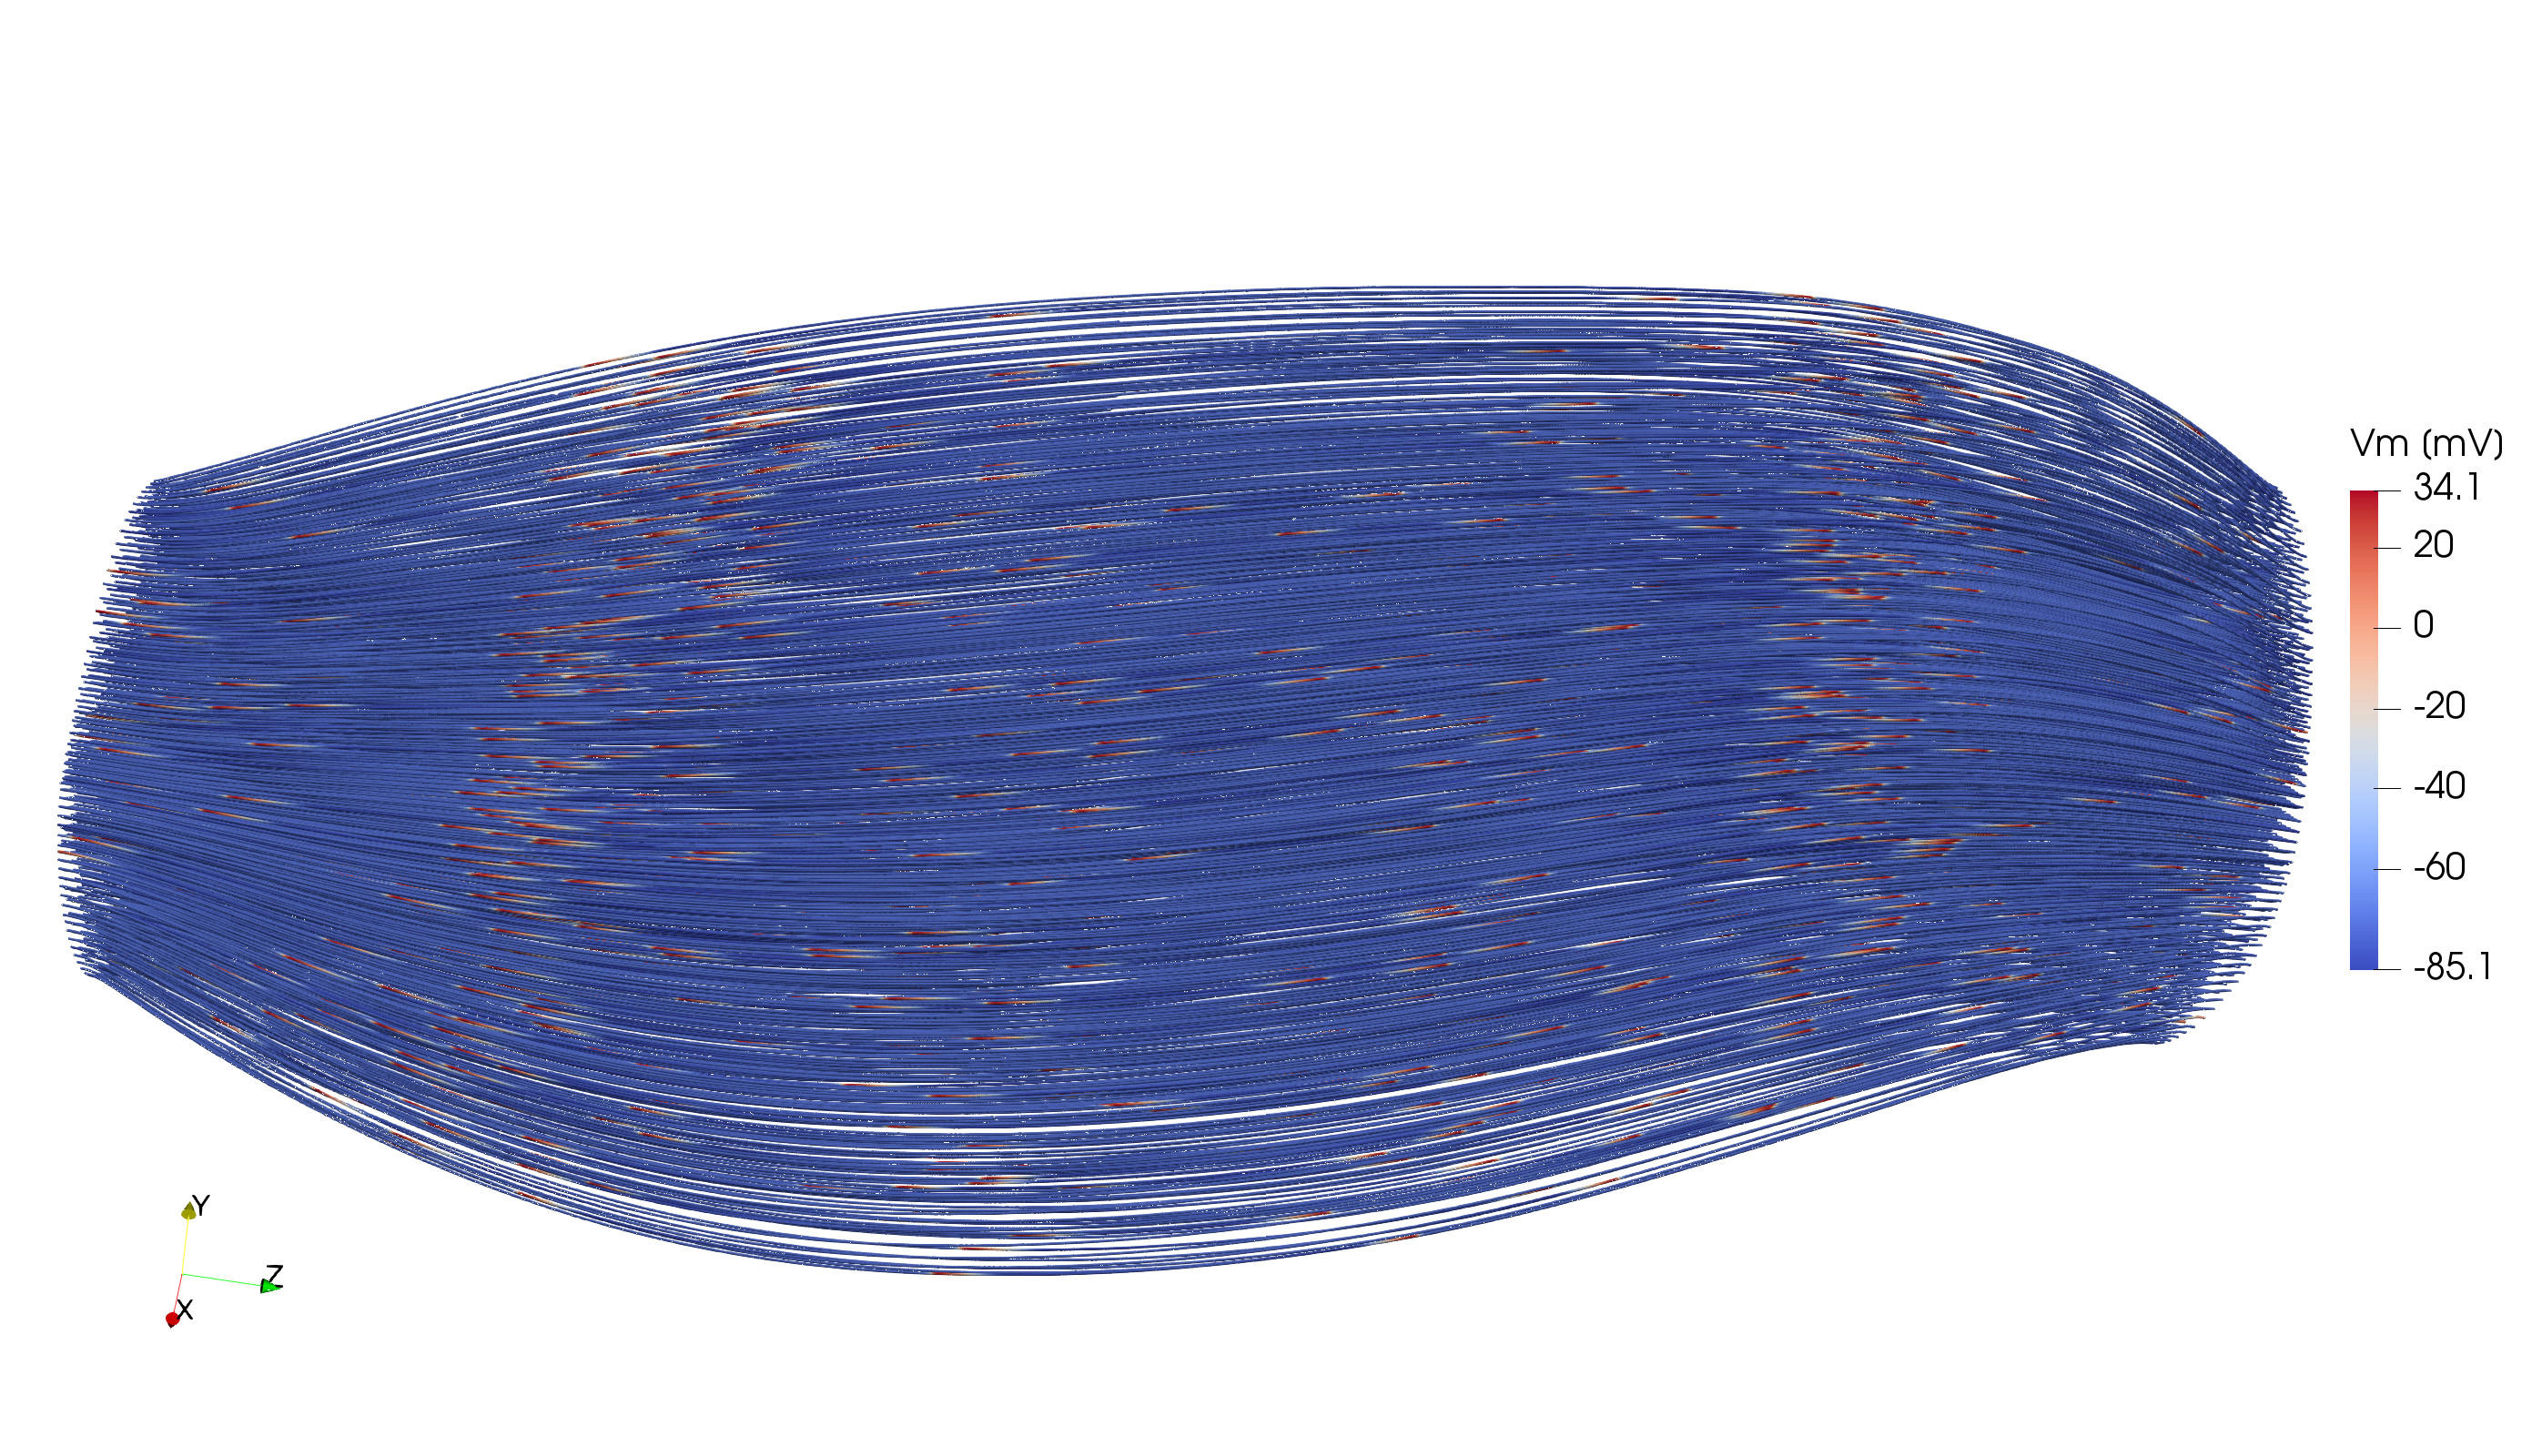
\includegraphics[width=\textwidth]{images/results/application/fibers_1.png}%
  \includegraphics[width=\textwidth]{images/results/application/fibers_2.png}%
  \caption{fibers mesh}%
  \label{fig:multidomain_mesh}%
\end{figure}

%-----
\section{Application: Motoneuron with fibers}
%-----
\section{Application: Rosenfalck, artifical muscle geometry}
%-----
\section{Application: Simulation of Monodomain Fibers with EMG}

% fibers mesh
\begin{figure}[H]
  \centering%
  \includegraphics[width=\textwidth]{images/results/application/fibers_3.png}%
  \includegraphics[width=\textwidth]{images/results/application/fibers_4.png}%
  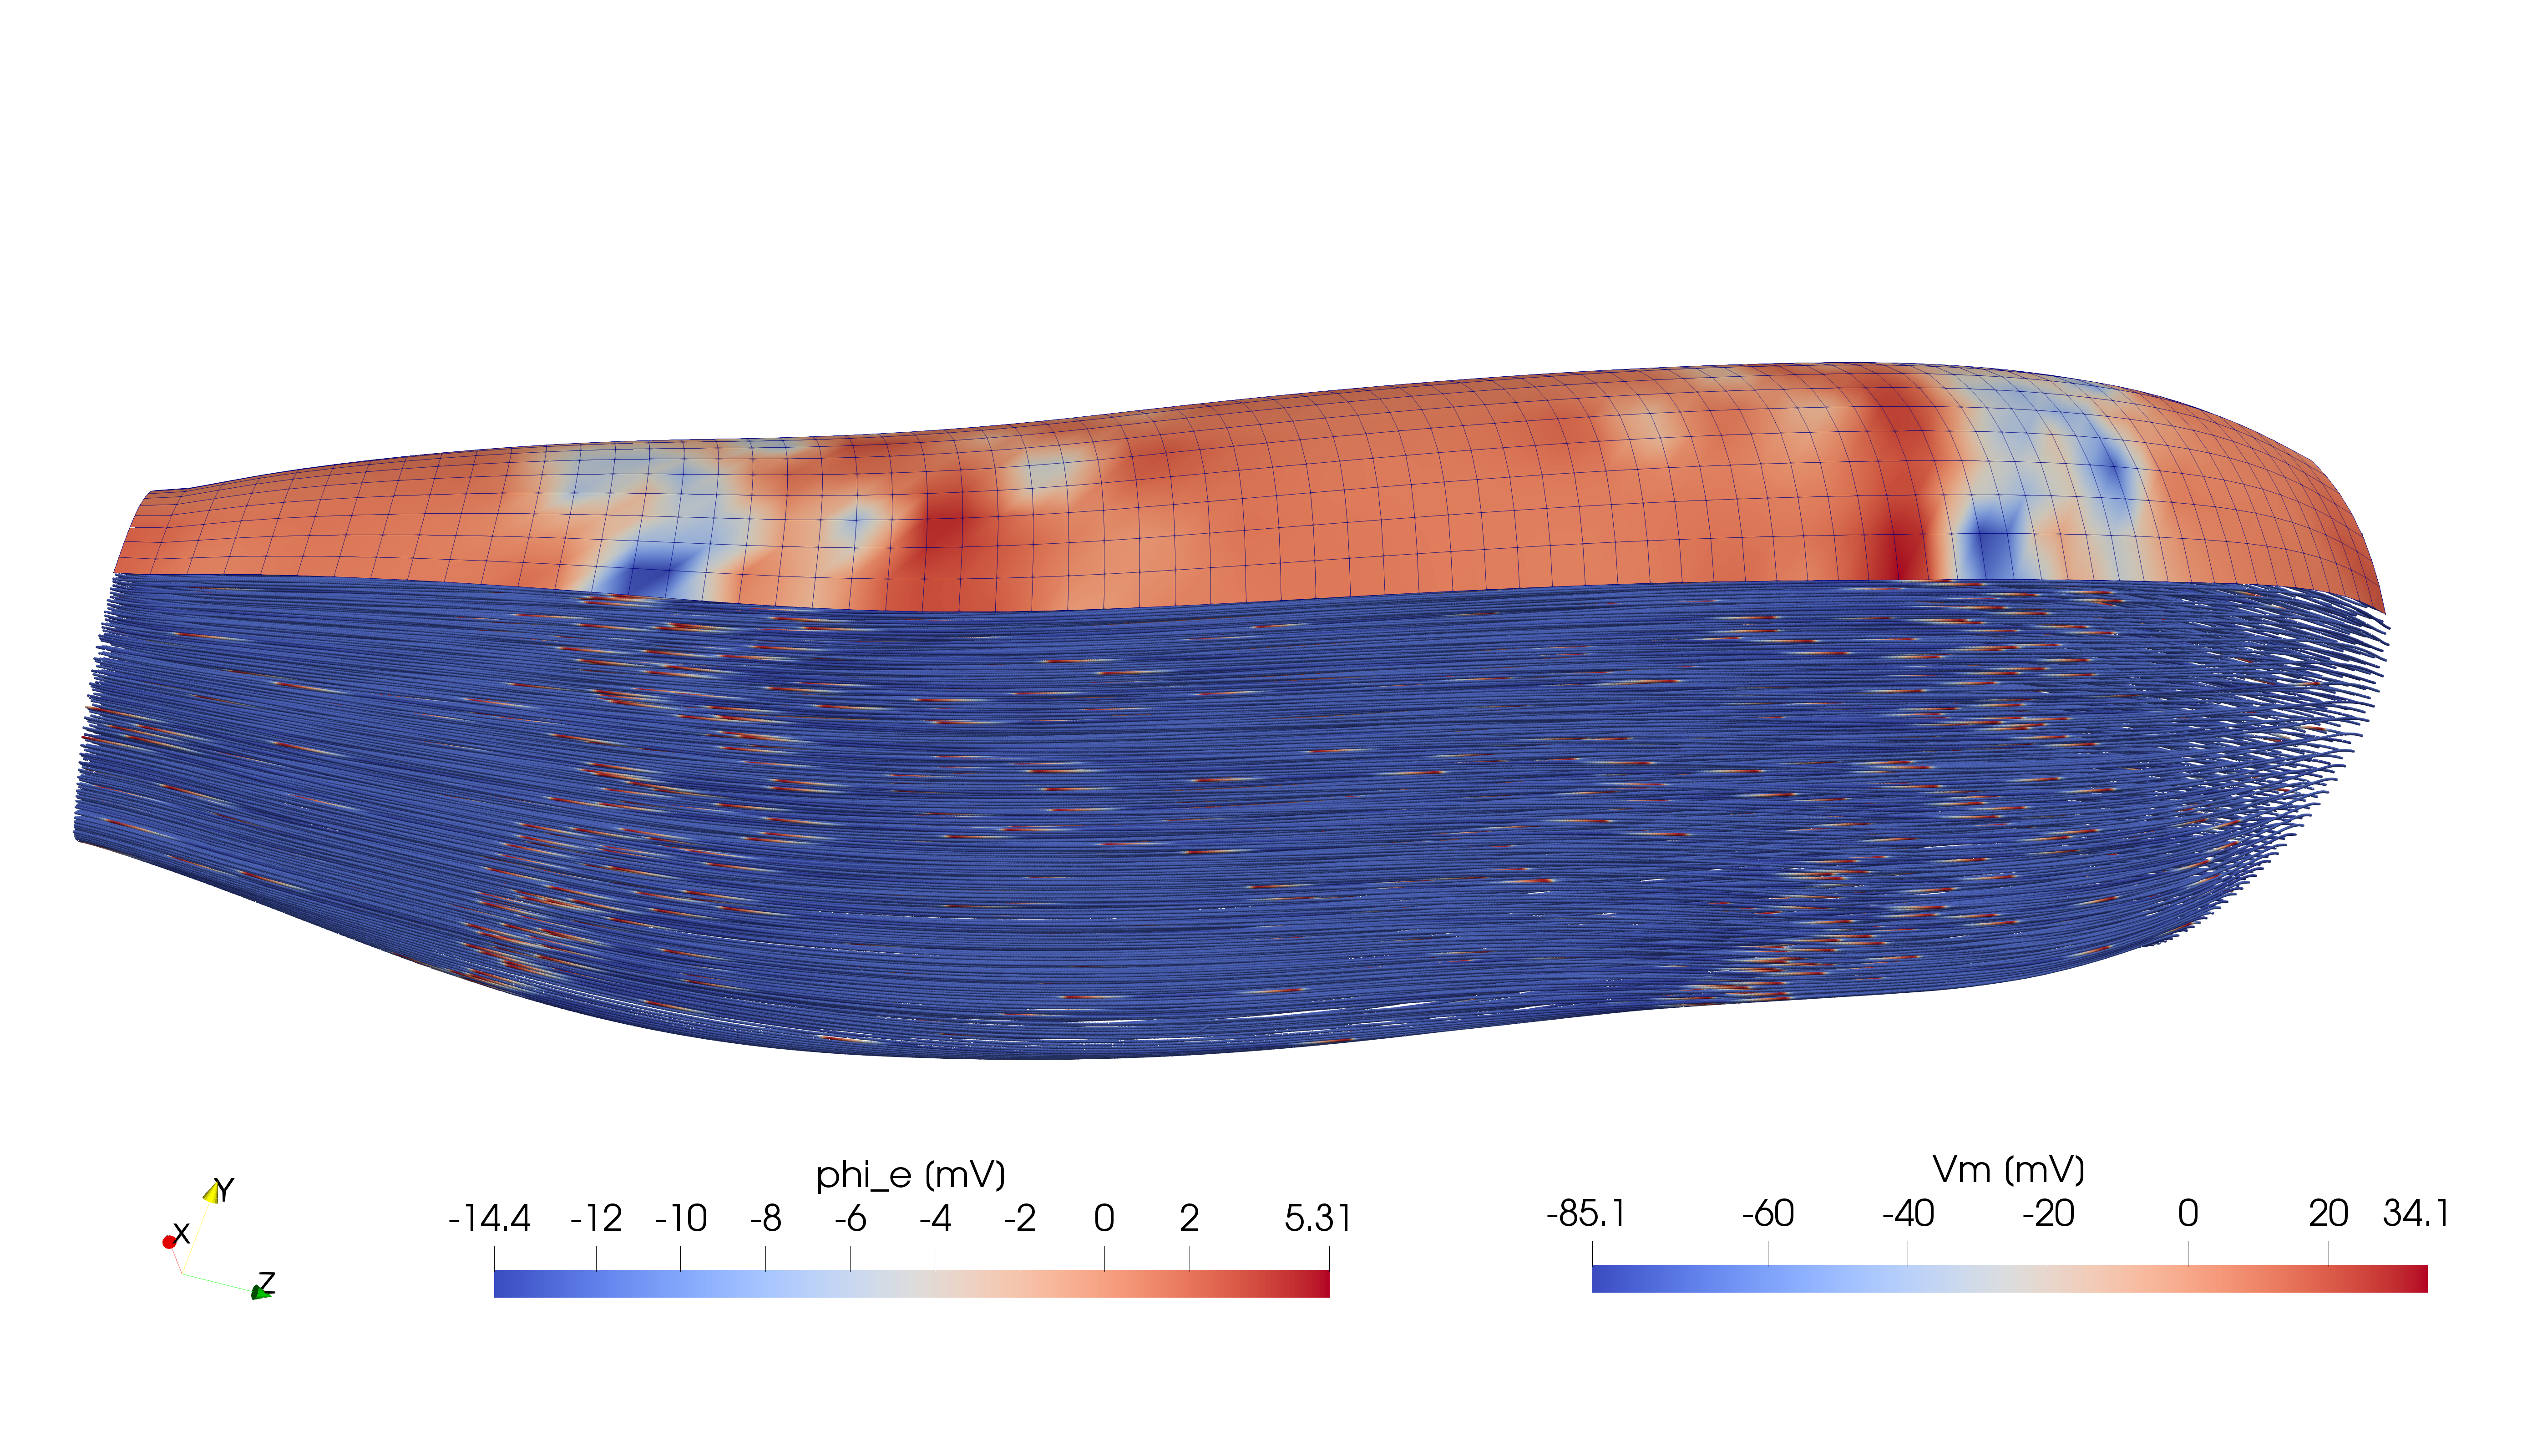
\includegraphics[width=\textwidth]{images/results/application/fibers_5.png}%
  \caption{fibers mesh}%
  \label{fig:multidomain_mesh}%
\end{figure}


% plot of emg from fibers
\begin{figure}[H]
  \centering%
  \includegraphics[width=\textwidth]{images/results/application/fibers_plot.png}%
  \caption{fibers}%
  \label{fig:fibers_plot}%
\end{figure}

% full_muscle_emg_raytrace_1.png
\begin{figure}[H]
  \centering%
  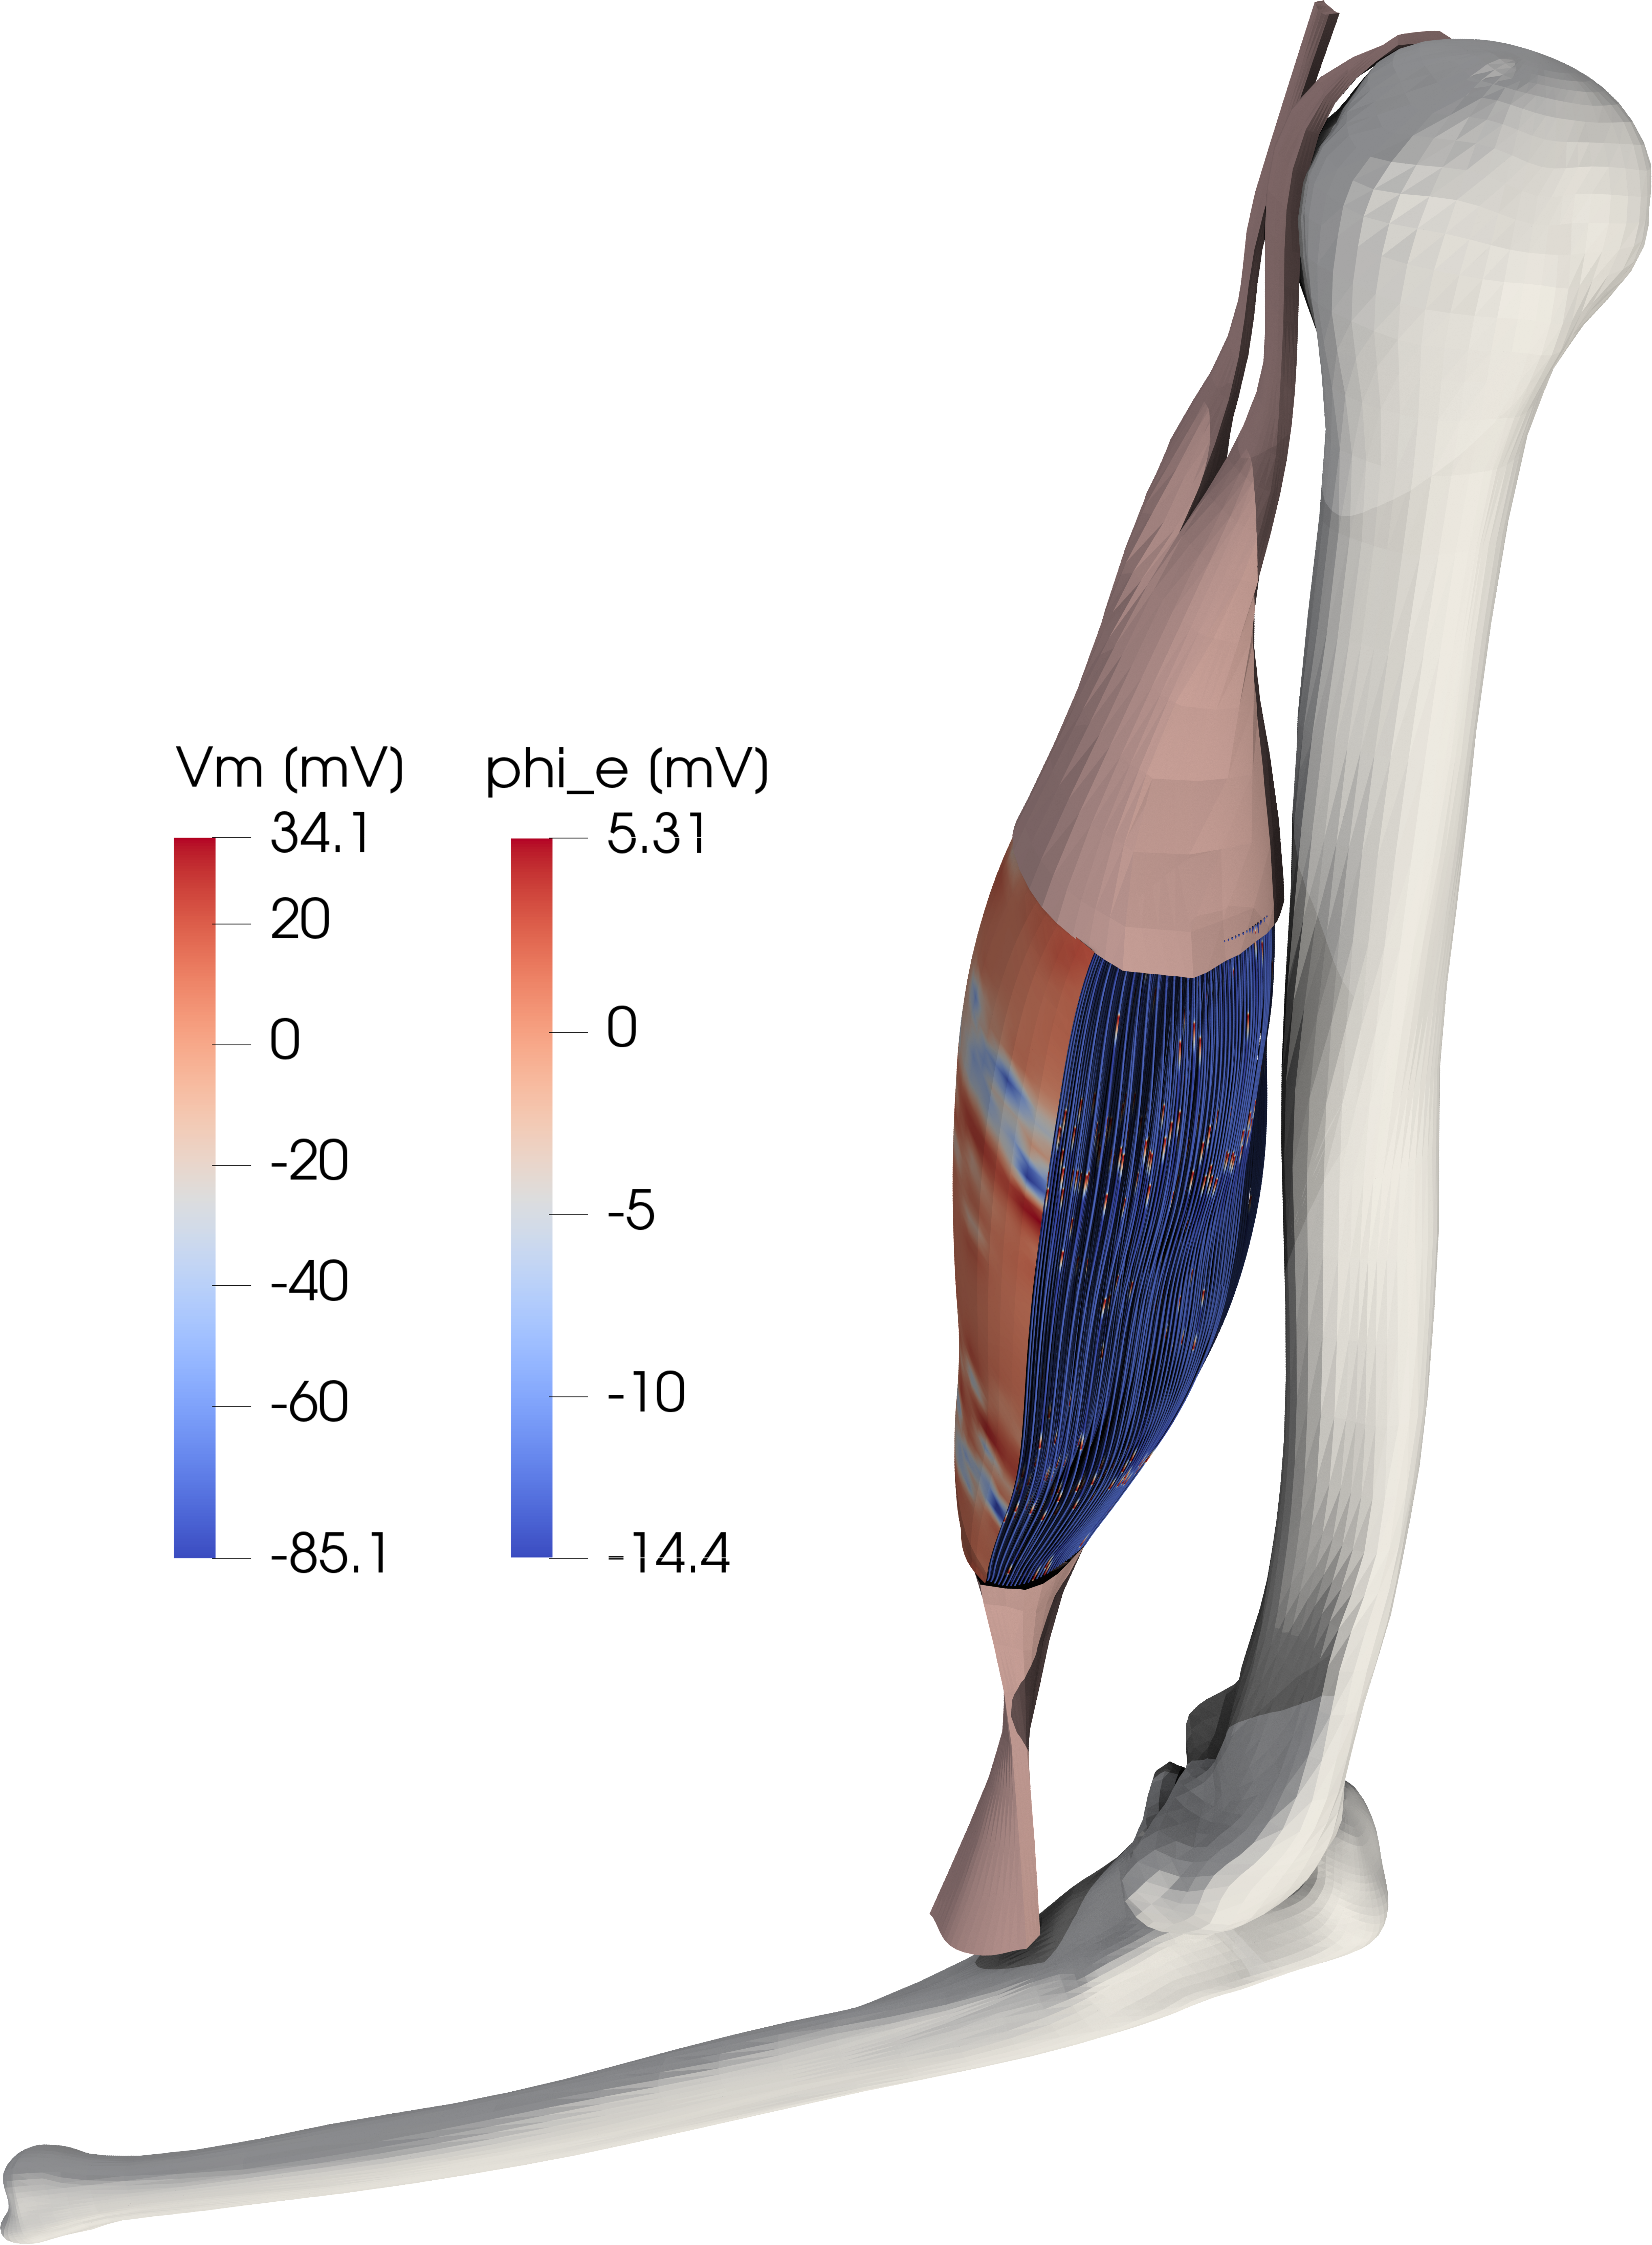
\includegraphics[width=\textwidth]{images/results/application/full_muscle_emg_raytrace_1.png}%
  \caption{muscle emg}%
  \label{fig:full_muscle_emg_raytrace_1}%
\end{figure}


%-----
\section{Application: Static bidomain}
%-----
\section{Application: Multidomain}


% multidomain fr factors
\begin{figure}[H]
  \centering%
  \begin{subfigure}[t]{0.23\textwidth}%
    \centering%
    \includegraphics[width=\textwidth]{images/results/application/multidomain_fr0_cropped.png}%
    \caption{$f_r^0$}%
    \label{fig:fr0}%
  \end{subfigure}
  \,
  \begin{subfigure}[t]{0.23\textwidth}%
    \centering%
    \includegraphics[width=\textwidth]{images/results/application/multidomain_fr1_cropped.png}%
    \caption{$f_r^1$}%
    \label{fig:fr1}%
  \end{subfigure}
  \,
  \begin{subfigure}[t]{0.23\textwidth}%
    \centering%
    \includegraphics[width=\textwidth]{images/results/application/multidomain_fr2_cropped.png}%
    \caption{$f_r^2$}%
    \label{fig:fr2}%
  \end{subfigure}
  \,
  \begin{subfigure}[t]{0.23\textwidth}%
    \centering%
    \includegraphics[width=\textwidth]{images/results/application/multidomain_fr3_cropped.png}%
    \caption{$f_r^3$}%
    \label{fig:fr3}%
  \end{subfigure}
\end{figure}%


% multidomain mesh
\begin{figure}[H]
  \centering%
  \includegraphics[width=\textwidth]{images/results/application/multidomain_mesh.png}%
  \caption{multidomain mesh}%
  \label{fig:multidomain_mesh}%
\end{figure}



% multidomain Vm
\begin{figure}[H]
  \centering%
  \begin{subfigure}[t]{\textwidth}%
    \centering%
    \includegraphics[width=\textwidth]{images/results/application/multidomain_Vm0_1.png}%
    \caption{$V_m^0$ and $V_m^1$}%
    \label{fig:16_hodgkin_huxley_gpu}%
  \end{subfigure} \\
  \begin{subfigure}[t]{\textwidth}%
    \centering%
    \includegraphics[width=\textwidth]{images/results/application/multidomain_Vm2_phi_b.png}%
    \caption{$V_m^2$ and $\phi_b$}%
    \label{fig:16_hodgkin_huxley_gpu}%
  \end{subfigure}   
  \caption{gpu.}%
  \label{fig:16_hodgkin_huxley_cpu_gpu}%
\end{figure}%

% fibers and multidomain
\begin{figure}[H]
  \centering%
  \begin{subfigure}[t]{0.48\textwidth}%
    \centering%
    \includegraphics[width=\textwidth]{images/results/application/2_multidomain.png}%
    \caption{Multidomain}%
    \label{fig:2_multidomain}%
  \end{subfigure}
  \quad
  \begin{subfigure}[t]{0.48\textwidth}%
    \centering%
    \includegraphics[width=\textwidth]{images/results/application/2_fibers.png}%
    \caption{Fibers}%
    \label{fig:2_fibers}%
  \end{subfigure}   
  \caption{Fibers and Multidomain}%
  \label{fig:multidomain_fibers}%
\end{figure}%


%-----
\section{Application: Linear mechanics with artifical electrophysiology}
%-----
\section{Application: Fibers and Muscle contraction, no-precice}
%-----

% prestretch
\begin{figure}[H]
  \centering%
  \includegraphics[width=0.5\textwidth]{images/results/application/fibers_muscle_contraction_quantities.png}%
  \caption{prestretch}%
  \label{fig:prestrech1b}%
\end{figure}%
\section{Application: Fibers and Muscle contraction, with tendons precice}

% muscle contraction
\begin{figure}
  \centering%
  \includegraphics[width=0.5\textwidth]{images/results/application/neuromuscular_muscle_contraction_traction.png}%
  \caption{solver structure}%
  \label{fig:neuromuscular_muscle_contraction_traction}%
\end{figure}%

%-----
\section{Application: Neuromuscular system with Spindles and Prestretch}

% prestretch
\begin{figure}[H]
  \centering%
  \includegraphics[width=0.5\textwidth]{images/results/application/neuromuscular_prestretch2c.png}%
  \caption{prestretch}%
  \label{fig:neuromuscular_prestretch2c}%
\end{figure}%

% image of contracting muscle
\begin{figure}[H]
  \centering%
  \includegraphics[width=\textwidth]{images/results/application/neuromuscular_contraction0.png}%
  \caption{Reference and current configuration.}%
  \label{fig:neuromuscular_contraction0}%
\end{figure}


% data flow of spindles
\begin{figure}[H]
  \centering%
  \includegraphics[width=\textwidth]{images/results/application/schematic_spindles.pdf}%
  \caption{Data flow of simulation with spindles and motor neurons}%
  \label{fig:neuromuscular_schematic}%
\end{figure}

% results
\begin{figure}[H]
  \centering%
  \includegraphics[width=\textwidth]{images/results/application/neuromuscular_spindle_out.png}%
  \caption{Activation data of sensors and neurons}%
  \label{fig:neuromuscular_schematic}%
\end{figure}

%-----
\section{Application: Neuromuscular system with More Sensor Organs}\label{sec:application_neuromuscular_system_more}

% data flow Golgi tendon organs
\begin{figure}[H]
  \centering%
  \includegraphics[width=\textwidth]{images/results/application/neuromuscular_schematic.pdf}%
  \caption{Data flow of simulation with spindles, Golgi tendon organs and motor neurons}%
  \label{fig:neuromuscular_schematic}%
\end{figure}

% results
\begin{figure}[H]
  \centering%
  \includegraphics[width=\textwidth]{images/results/application/neuromuscular_mileusnic_out0.png}\\
  \includegraphics[width=\textwidth]{images/results/application/neuromuscular_mileusnic_out1.png}\\
  \caption{Activation data of sensors and neurons}%
  \label{fig:neuromuscular_schematic}%
\end{figure}

\fi
% --------------------------------
% studies, performance
%-----
%\section{Strang Splitting}
%-----
\iffalse
\section{Performance Studies with OpenCMISS Iron}

Next, we study the performance of the software by evaluating runtimes and parallel scalability for different solvers.
We begin with OpenCMISS Iron as the baseline solver that also implements parts of the multi-scale model considered in this work. The work of \cite{Heidlauf2013} describes the implementation of the fiber based electrophysiology model coupled to a quasi-static hyperelastic material model with OpenCMISS. The implementation is parallelized for a hardcoded number of four processes and serves as the baseline code for the following studies.

We improved the performance of this solver for the multi-scale model by two actions: First, we evaluated and optimized the employed numeric schemes. Second, we implemented parallel partitioning for an arbitrary number of processes and evaluated different parallelization strategies.
These changes were directly implemented in the OpenCMISS code. The improvements were also presented in a publication \cite{Bradley:2018:EDB}. In the following sections \cref{sec:opencmiss_numeric_improvements,sec:opencmiss_parallel_partitioning}, we describe the numeric improvements and the parallel partitioning strategies. In \cref{sec:opencmiss_memory}, we discuss the parallel weak scaling and memory consumption properties.

\subsection{Numeric Improvements}\label{sec:opencmiss_numeric_improvements}

The first numeric improvement is to replace the GMRES solver that is used to solve the 1D electric conduction problem on the muscle fibers
by a faster direct solver. 

As noted in \cref{sec:improved_parallel_solver_for_fiber_based}, the 1D electric conduction problem of the monodomain equation yields a tridiagonal system that can be solved with linear time complexity. The baseline solver code employs the restarted GMRES solver of PETSc, which is the default linear system solver in OpenCMISS Iron, as it is a robust choice for abitrary system matrices. 
More efficient solvers exist for symmetric positive definite systems such as the conjugate gradient scheme. 
Furthermore, the MUMPS package \cite{mumps2001} that can be interfaced in PETSc provides a parallel implementation of a direct, multi-frontal linear solver, which is able to exploit banded structures of the system matrix.

We study the runtime of these three solvers for different problem sizes of the 1D problem. The monodomain equation is solved on a single muscle fiber and the number of 1D elements is varied from 15 to 2807. The used timestep widths are $\dt_\text{0D}=\SI{1e-4}{\ms}$ and $\dt_\text{1D}=\SI{5e-3}{\ms}$. The end time of the simulation is $\SI{3}{\ms}$, yielding a total number of 600 solutions of the linear system. The study is executed on an Intel Xeon E7540 processor with 24 cores, clock frequency of \SI{1064}{\mega\hertz} and \SI{506}{\gibi\byte} RAM.

\Cref{fig:opencmiss_linear_solvers} shows the runtime of the GMRES, conjugate gradient and direct solvers for this problem in a double-logarithmic plot.
It can be seen, that, for coarse discretizations with a low number of 1D elements per fiber, the GMRES and conjugate gradient solvers are faster than the direct solver. For finer discretizations, the conjugate gradient solver and the direct solver outperform the GMRES solver. For fibers with more than approximately 500 elements, the direct solver has the lowest runtime. Moreover, the direct solver exhibits an almost linear runtime complexity in terms of the problem size. This indicates that the solver is able to exploit the tridiagonal structure of the system matrix.

% linear solvers plot
\begin{figure}
  \centering%
  \includegraphics[width=0.9\textwidth]{images/results/studies/opencmiss_linear_solvers.pdf}%
  \caption{Numeric improvements in OpenCMISS: Runtime evaluation of different linear system solvers for a single muscle fiber with varying spatial resolution.}%
  \label{fig:opencmiss_linear_solvers}%
\end{figure}%

The second numeric improvement is the exchange of first-order accurate timestepping schemes by second-order schemes. For this exchange, we implemented the Strang operator splitting scheme and use it with the existing Crank-Nicolson implementation in OpenCMISS Iron and the Heun method, which was  implemented by Aaron Krämer.

Numerical studies by Aaron Krämer presented in \cite{Bradley:2018:EDB} show that the relation $K=\dt_\text{1D}/\dt_\text{0D}$ between the timestep width $\dt_\text{1D}$ of the 1D electric conduction problem and the timestep width $\dt_\text{0D}$ of the 0D subcellular model has to be set to $K=2$ and $K=5$ for the Godunov and Strang splitting schemes, respectively, such that the errors of the 0D and 1D subproblems are balanced. To achieve a total error for the membrane potential $V_m$ of approximately \num{8e-2}, we can increase the required splitting timestep width $\dt_\text{splitting}$ from $\SI{5e-4}{\ms}$ for the Godunov splitting to $\SI{4e-3}{\ms}$ for the Strang splitting scheme. This results in a runtime speedup  of approximately 7.5.

To evaluate the total speedup of the described numeric improvements, we compare the runtimes without and with the improvements for a complete simulation of the fiber based electrophysiology model coupled with the elasticity model. A cuboid 3D domain is discretized by $2\times 2\times 2=8$ finite elements for the elasticity model and embeds $6\times 6=36$ 1D fiber meshes. The number of 1D elements per fiber is varied between 576 and \num{239400} to study the scaling behavior of the solvers depending on the problem size. The problem is solved in serial to avoid effects introduced by the parallelization.

The baseline implementation uses the Godunov splitting with forward and implicit Euler schemes for the 0D subcellular model and the electric conduction model, respectively. The linear system in the 1D problem is solved by a GMRES solver with relative residuum tolerance of \num{1e-5} and restart after 30 iterations. Timestep widths of $\dt_\text{0D}=\SI{1e-4}{\ms}$ and $\dt_\text{splitting}=\dt_\text{1D}=\SI{5e-4}{\ms}$ are used. The improved scheme uses the Strang operator splitting with Heun and Crank-Nicolson schemes and timestep widths of $\dt_\text{0D}=\SI{2e-3}{\ms}$ and $\dt_\text{splitting}=\dt_\text{1D} = \SI{4e-3}{\ms}$. The direct solver is used for the linear system in the 1D problem.
The solver for the 3D elasticity problem is the same for both implementations. A Newton scheme with residual tolerance of \num{1e-8} is used
 and coupled to the 0D and 1D solvers with a coupling timestep width of $\dt_\text{3D}=\SI{1}{\ms}$.

The present study and the studies in the next section are executed on the supercomputer \emph{Hazel Hen} at the High Performance Computing Center Stuttgart. This Cray XC40 system contains compute nodes with two Intel Haswell E5-2680v3 processors with a base frequency of \SI{2.5}{\giga\hertz}, 12 cores per CPU, 24 cores per compute node and \SI{128}{\giga\byte} RAM per node.

% improvements plot
\begin{figure}
  \centering%
  \includegraphics[width=\textwidth]{images/results/studies/opencmiss_cuboid_serial_scaling_comparison_aggressive.pdf}%
  \caption{Numeric improvements in OpenCMISS: Study to evaluate the speedup of the improved implementation of the fiber-based electrophysiology and mechanics model in OpenCMISS.}%
  \label{fig:opencmiss_improvements}%
\end{figure}%
% 576.0, 792.0, 1224.0, 1872.0, 2736.0, 4176.0, 6192.0, 9360.0, 14040.0, 21024.0, 31536.0, 47304.0, 70920.0, 106416.0, 159624.0, 239400.0

\Cref{fig:opencmiss_improvements} shows the results of this study. In the upper part, the runtimes for different components of the simulation are indicated by different colors in a plot with double logarithmic scale. The runtimes for the baseline implementation are shown by solid lines and the runtimes including the improvements are shown by dashed lines. In the lower plot, the speedups from the baseline to the improved implementation are given.

The total runtime of the simulation is given by the black lines in the upper plot. It can be seen that the total runtime results almost completely from the 0D model solver, which is shown by the yellow lines. The 1D solver, given by the red lines, has the second most influence. The effects of the data mapping operations between the 3D mesh and the 1D fibers on the runtime are negligible. These data mapping operations consists of the homogenization step from the 1D fibers to the 3D mesh and the interpolation step from the 3D mesh to the 1D fibers.

The runtimes for almost all problem parts increase linearly for increasing mesh resolution of the 1D fibers. Only the runtime of the 3D problem stays constant, as the 3D mesh is unchanged for the different runs.

Significant runtime improvements of the new implementation compared to the baseline implementation can be seen in the lower plot of   \cref{fig:opencmiss_improvements} for the 0D solver and the 1D solver. The speedup for the 0D solver is constant at approximately 2.5. The speedup resulting from the improved linear system solver in the 1D problem is approximately 6.1 for coarse meshes and increases to 14.7 for the finest mesh. This increase for high mesh resolutions results from the higher runtime of the GMRES solver for large problem sizes in the baseline implementation. The overall speedup is similar to the speedup of the 0D problem, as the 0D solver is responsible for the most runtime of the computation.

This study shows how numeric investigations can help to reduce the total runtime, in this case by a factor of 2.5. Moreover, the solver of the 0D model has the most potential to further speed up computation times.

\subsection{Parallel Partitioning Strategies}\label{sec:opencmiss_parallel_partitioning}

To exploit parallelism and, thus, further reduce the computation times, we implemented a generic domain decomposition for the studied problem in OpenCMISS Iron.
Like in OpenDiHu, the 3D mesh can be partitioned to an arbitrary number of $n_x \times n_y \times n_z$ subdomains. The embedded 1D fibers are aligned with the $z$ axis and are partitioned by the same cut planes as the 3D mesh.

% pillars-cubes visualization
\begin{figure}[H]
  \centering%
  \begin{subfigure}[t]{0.48\textwidth}%
    \centering%
    \def\svgwidth{0.7\textwidth}
    \input{images/results/studies/opencmiss_ddpillar.pdf_tex}%
    \caption{\say{Pillar-like} domain decomposition with $n_z=1$.}%
    \label{fig:opencmiss_ddpillar}%
  \end{subfigure}
  \quad
  \begin{subfigure}[t]{0.48\textwidth}%
    \centering%
    \def\svgwidth{0.7\textwidth}
    \input{images/results/studies/opencmiss_ddcube.pdf_tex}%
    \caption{\say{Cube-like} domain decomposition}%
    \label{fig:opencmiss_ddcube}%
  \end{subfigure}   
  \caption{Different parallelization strategies that are implemented in the OpenCMISS model. This figure shows two approaches how the domain can be partitioned to 16 subdomains.}%
  \label{fig:opencmiss_dd_annotated}%
\end{figure}%

\Cref{fig:opencmiss_dd_annotated} shows two exemplary partitionings. If the domain is only partitioned in $x$ and $y$ directions, the fibers are not split into multiple subdomains. As a result, we get \say{pillar} subdomains as shown in \cref{fig:opencmiss_ddpillar}. An alternative approach is to subdivide the domain in all three coordinate directions such that the subdomains are approximately cube shaped, as shown in \cref{fig:opencmiss_ddcube}.

OpenCMISS Iron already provides the functionality to create partitioned unstructured meshes. However, every mesh has to be partitioned into non-empty subdomains for all processes. Thus, it is not possible to use individual meshes for the 1D fibers.
In the baseline implementation of the model by \cite{Heidlauf2013}, all 1D fiber meshes are instead realized as a single mesh, whose node positions are set according to the positions of the individual fibers. This facilitates the implementation of the 0D subcellular model solvers and 1D model solvers, as the implementation has to deal with only a single mesh. 

To allow for an arbitrary partitioning as in \cref{fig:opencmiss_dd_annotated}, we assigned the 1D elements of the single fiber mesh to the same processes as the subdomains of the 3D mesh. Furthermore, we reimplemented the data mapping between the 1D mesh and the 3D mesh, which was hardcoded for four processes.

In the following, we investigate the effect of different partitioning strategies on the overall runtime of the solver. The idea is that, for pillar-like partitionings as in \cref{fig:opencmiss_ddpillar}, the 1D problems could potentially be solved faster, as the fibers, which are aligned in $z$-direction, are not subdivided to multiple processes. On the other hand, the partitioning to cubes in \cref{fig:opencmiss_ddcube} requires less communication in the solution of the 3D problem as the cubes minimize the surface of each subdomain and, in consequence, the amount of data to be exchanged. We evaluate how these effects influence the runtime for the pillar-like partitioning, the cube partitioning and all other possible partitionings specified by numbers of subdomains $n_x \times n_y \times n_z$.

Our test case uses a 3D mesh with $12 \times 12 \times 144$ elements. To reduce the runtime contribution of the 0D/1D electrophysiology problem and the memory consumption of the solver, only two 1D elements per 3D element are included. The numeric parameters are the same as for the improved scenario presented in \cref{fig:opencmiss_improvements}. The simulations are executed on 12 compute nodes of the supercomputer Hazel Hen with 12 processes per node.

We partition the 3D domain to 144 processes using different combinations of $n_x,n_y$ and $n_z$ such that $n_x\,n_y\,n_z=144$. 
For every partitioning, we compute the average surface area of the boundary of every subdomain. 
\Cref{fig:opencmiss_partition_shape} shows the resulting runtime in relation to this average boundary area.
The pillar-like partitioning uses $12 \times 12 \times 1$ subdomains and exhibits the largest boundary surface area, corresponding to the last point in \cref{fig:opencmiss_partition_shape}. The cube partitioning consists of $6 \times 6 \times 4$ subdomains and corresponds to the first data point with the smallest boundary area.

% plot of partition shapes
\begin{figure}
  \centering%
  \includegraphics[width=\textwidth]{images/results/studies/opencmiss_partition_shape.png}%
  \caption{Runtime of the solvers for different partition shapes, from cube partitions on the left to pillar partitions on the right.  \footnotesize(This figure has also been published in \cite{Bradley:2018:EDB} under a creative commons license.)}%
  \label{fig:opencmiss_partition_shape}%
\end{figure}%

The plot shows that the runtime of the 3D solver increases approximately linearly with the amount of communication, which is expected.
The partitioning with the largest average surface area has a runtime that is approximately four times as large as the runtime for the smallest surface area.

Moreover, the plot shows that the partitioning scheme has no significant influence on the runtime of the 1D solver. The reason is that the implementation does not fully reflect the decoupled nature of the individual problems of the fibers. As noted before, one big linear system has to be solved that contains the degrees of freedom of all fibers. The degrees of freedom are ordered by PETSc such that the nodes within every subdomain are consecutive. If a subdomain contains (parts of) multiple fibers, their degrees of freedom are not necessarily consecutive in the solution vector and communication is required.

\subsection{Weak Scaling Study and Memory Consumption}\label{sec:opencmiss_memory}

Next, we evaluate the parallel weak scaling properties of the overall solver. We increase the number of elements in the 3D mesh from 1232 to 8640 and the total number of 1D elements in all fibers from \num{14784} to \num{103680}. Correspondingly, the number of processes increases from 24 to 192, such that the amount of work per process stays approximately constant. Each scenario is computed with two different partitioning schemes, once with a pillar-like partitioning and once with a cube partitioning. For the exact problem sizes, numbers of cores and numbers of elements in the partitions, we refer to the paper \cite{Bradley:2018:EDB}. 

% weak scaling runtime
\begin{figure}
  \centering%
  \includegraphics[width=\textwidth]{images/results/studies/opencmiss_weak_scaling.png}%
  \caption{Parallel weak scaling study of a scenario with the pillars and cubes partitionings.  \footnotesize(This figure has also been published in \cite{Bradley:2018:EDB} under a creative commons license.)}%
  \label{fig:opencmiss_weak_scaling}%
\end{figure}

\Cref{fig:opencmiss_weak_scaling} shows the resulting runtimes of the different components of the simulation. It can be seen that the runtime stays approximately the same for all problem sizes. The observable differences in runtime within the same solver, especially for the last two data points, can be explained by a slighly different ratio of element count to process count, which results from the goal to use the pillar and cubes partitioning schemes while not exceeding the available main memory.

The runtimes of the pillars and cubes partitioning schemes are depicted by dashed and solid lines, respectively. The pillars partitioning exhibits shorter runtimes for the 1D solver and longer runtimes for the 3D solver compared to the cubes partitioning. In total, the runtime is not significantly different for the different partitioning strategies.

% memory consumption
\begin{figure}
  \centering%
  \includegraphics[width=\textwidth]{images/results/studies/opencmiss_memory.png}%
  \caption{Memory consumption per process at the end of the simulation corresponding to the weak scaling study of \cref{fig:opencmiss_weak_scaling}. \footnotesize(This figure has also been published in \cite{Bradley:2018:EDB} under a creative commons license.)}%
  \label{fig:opencmiss_memory}%
\end{figure}%

A limiting factor for the construction of weak scaling studies with this implementation is the high memory consumption. \Cref{fig:opencmiss_memory} shows the total memory consumption per process at the end of the runtime of the simulations in \cref{fig:opencmiss_weak_scaling}. The used memory is visualized by purple lines. The dashed line again corresponds to the pillars partitioning and the solid line corresponds to the cubes partitioning. 

As can be seen, the memory consumption per process monotonically increases with the total number of 1D elements. 
At the same time, however, the number of elements per process stays approximately constant in this weak scaling setting. The last data point is close to the memory limit of $\SI{128}{\giga\byte} / 24 \approx \SI{4.967}{\gibi\byte}$, which is reached when 24 processes are executed on a compute node of the supercomputer Hazel Hen.

A difference between the pillar partitions and the cube partitions is the size of the subdomain surfaces and the corresponding size of the ghost layer. \cref{fig:opencmiss_memory} shows the number of 3D ghost elements for the scenarios with cubes and pillars by the black lines. In OpenCMISS, a ghost element on a process is an element that contains ghost nodes, which are owned by a different process. The ghost elements serve as data buffers for communication during the assembly of the finite element matrices, similar to OpenDiHu.

The plot in \cref{fig:opencmiss_memory} shows that the number of ghost elements is higher for the pillar partitioning scheme than for the cubes scheme, as expected. In consequence, the memory consumption per process is also slightly higher for the pillar partitioning.
However, this effect is negligible compared to the high absolute value of the required memory and does not explain this effect.

The increase in memory results from the organization of parallel partitioned data in OpenCMISS Iron. On every process, global mesh topology information such as mappings between global indexing and local indexing is stored for the element numbers, node numbers and degree of freedom numbers. While this overhead in storage is negligible for moderately parallel scenarios, it counteracts the domain decomposition approach for higher degrees of parallelism. 

Numerous functions and algorithms in the OpenCMISS Iron code rely on this type of global information. Thus, eliminating the parallelism constraint by reorganizing the data structures is a highly involved task. Especially the initialization of the parallel partitioning heavily uses this global information. This initialization includes, e.g., the distribution of elements and nodes to the subdomains on the processes, the determination of the ghost layers and dofs to send to and receive from neighbor processes, and the setup of local numbers for elements, nodes and degrees of freedom.

We addressed the elimination of this use of global topology information in the initialization steps and developed and implemented appropriate local algorithms in OpenCMISS Iron. This resulted in major code changes that are difficult to oversee, also because of the lacking object orientation in the code base and the difficulty to test the functionality. Creating the required comprehensive set of unit tests for nearly all functionality of OpenCMISS would be a large task that remains to be done. Thus, these code changes could not be merged into the main trunk of OpenCMISS.

Even with these code changes, the memory problem is not yet solved. Another problem prior to the initialization step is that the mesh has to be specified from the user code in a global data structure. It is currently not possible to specify a mesh in a distributed way. Thus, OpenCMISS Iron can only use meshes that initially fit into the main memory on a single core.

Moreover, another issue is concerned with the data structures for matrices. Each process stores its local row indices and additionally a map from global to local row indices for all dofs of the global problem. This global-to-local map also contributes to the bad weak memory scaling and has to be eliminated as well. One possible approach is to use hash maps and only store the relevant portion of the mapping on every process. Work towards resolving this issue has been started by Lorenzo Zanon at the former SimTech Research Group on Continuum Biomechanics and Mechanobiology at the University of Stuttgart. 

One reason for the generic mapping of matrix rows, which uses global information, is that OpenCMISS Iron does not restrict discretization schemes to the finite element method, where the system matrix can be assembled from local element matrices within the subdomains. An example for a different scheme is the boundary element method.

In addition, there exist more parts in the code that use a similar global-to-local mapping and would also have to be changed to allow for a constant memory consumption per process, e.g, the boundary condition handling and the data mapping between the 3D mesh and the fibers.

In summary, fixing the issue of non-scaling memory consumption in OpenCMISS Iron corresponds to redeveloping a significant portion of the code. 
To preserve the generic functionality of OpenCMISS, some changes would require new algorithmic considerations and complex workarounds.
This development effort would have to be quick enough to keep up with the independent development of the normal OpenCMISS branch. After completion, the merge back into the main software trunk would only be possible if the branches had not diverged too far and after significant efforts have been put into testing and preserving the feature set of OpenCMISS.

On the other hand, developing the missing functionality from scratch and making sensible restrictions on the generality of the solved problems and used methods requires possibly less effort and allows to consider design goals such as performance, usability and extensibility from the beginning.
In this sense, the OpenDiHu software project can be seen as a complement to OpenCMISS Iron.  %companion
The mentioned restrictions are, e.g., the exclusive use of the finite element method and cartesian coordinates and the use of parallel partitioned structured meshes instead of the more complex parallelization of unstructured meshes.
\fi

%-----
\section{Monodomain Solver Performance}

% fibers_emg performance
\begin{figure}
  \centering%
  \includegraphics[width=\textwidth]{images/results/studies/fibers_emg_study.pdf}%
  \caption{Efficiency model}%
  \label{fig:fibers_emg_study}%
\end{figure}%

% fibers_emg performance shorten
\begin{figure}
  \centering%
  \includegraphics[width=\textwidth]{images/results/studies/fibers_emg_study_shorten.pdf}%
  \caption{Efficiency model shorten}%
  \label{fig:fibers_emg_study_shorten}%
\end{figure}%

\iffalse
% 0/18 : This is opendihu 1.2, built Apr  9 2021, C++ 201703, GCC 10.2.0, current time: 2021/4/9 17:15:06, hostname: pcsgs05, n ranks: 18                                                       
% 0/18 : Open MPI v3.1.6, package: Open MPI maierbn@sgscl1 Distribution, ident: 3.1.6, repo rev: v3.1.6, Mar 18, 2020                                                                           
% 0/18 : File "../settings_fibers_emg.py" loaded.                                                                                                                                               
% 0/18 : ---------------------------------------- begin python output ----------------------------------------                                                                                  
% Loading variables from "ramp_emg.py".                                                                                                                                                         
% scenario_name: fast-vc,  n_subdomains: 3 2 3,  n_ranks: 18,  end_time: 10.0
% dt_0D:           3.0e-03, diffusion_solver_type:      cg                                                                                                                                      
% dt_1D:           1.0e-03, potential_flow_solver_type: gmres, approx. exp.: False                                                                                                              
% dt_splitting:    3.0e-03, emg_solver_type:            cg, emg_initial_guess_nonzero: False                                                                                                    
% dt_3D:           4.0e-01, paraview_output: True, optimization_type: vc (AoVS)                                                                                                                 
% output_timestep: 4.0e+05, surface: 1.0e+00, stimulation_frequency: 0.1 1/ms = 100.0 Hz                                                                                                        
%                           fast_monodomain_solver_optimizations: False                          
% fiber_file:              ../../../input/left_biceps_brachii_25x25fibers.bin                                                                                                                   
% cellml_file:             /data/scratch/maierbn/opendihu/examples/electrophysiology/input/hodgkin_huxley_1952.c                                                                                
% fiber_distribution_file: /data/scratch/maierbn/opendihu/examples/electrophysiology/input/MU_fibre_distribution_10MUs.txt                                                                      
% firing_times_file:       /data/scratch/maierbn/opendihu/examples/electrophysiology/input/MU_firing_times_always.txt                                                                           
% ********************************************************************************                                                                                                              
% prefactor: sigma_eff/(Am*Cm) = 0.03079310344827586 = 8.93 / (500.0*0.58)                                                                                                                      
% diffusion solver type: cg                                                                                                                                                                     
% n fibers:              625 (25 x 25), sampled by stride 2 x 2                                  
% n points per fiber:    1481, sampled by stride 50                                                                                                                                             
% 18 ranks, partitioning: x3 x y2 x z3                                                                                                                                                          
% 25 x 25 = 625 fibers, per partition: 8 x 12 = 96                                                                                                                                              
% per fiber: 1D mesh    nodes global: 1481, local: 500                                           
%   sampling 3D mesh with stride 2 x 2 x 50                                                      
%     linear 3D mesh    nodes global: 13 x 13 x 31 = 5239, local: 4 x 6 x 10 = 240               
%     linear 3D mesh elements global: 12 x 12 x 30 = 4320, local: 4 x 6 x 10 = 240               
% number of degrees of freedom:                                                                  
%                     1D fiber:       1481  (per process: 500)                                   
%             0D-1D monodomain:       5924  (per process: 2000)                                  
%  all fibers 0D-1D monodomain:    3702500  (per process: 192000)                                                                                                                               
%                  3D bidomain:       5239  (per process: 240)                                   
%                        total:    3707739  (per process: 192240)                                                                                                                               
% Python config parsed in 0.1s.        
% 0/18 : ----------------------------------------- end python output -----------------------------------------                                                                                  
% 0/18 : Read from file "../../../input/left_biceps_brachii_25x25fibers.bin", 502 collective chunks.                                                                                            
% done.                                                              

% -----------------------------------------------------------------------------------------------------
% shorten:
% ===== vc 2 =====                   
% 0/18 : This is opendihu 1.2, built Apr  9 2021, C++ 201703, GCC 10.2.0, current time: 2021/4/9 17:50:15, hostname: pcsgs05, n ranks: 18                                                       
% 0/18 : Open MPI v3.1.6, package: Open MPI maierbn@sgscl1 Distribution, ident: 3.1.6, repo rev: v3.1.6, Mar 18, 2020                                                                           
% 0/18 : File "../settings_fibers_emg.py" loaded.   
% 0/18 : ---------------------------------------- begin python output ----------------------------------------                                                                                  
% Loading variables from "shorten.py".                                                           
% scenario_name: vc-aovs,  n_subdomains: 3 2 3,  n_ranks: 18,  end_time: 3.0
% dt_0D:           2.5e-05, diffusion_solver_type:      cg
% dt_1D:           2.5e-05, potential_flow_solver_type: gmres, approx. exp.: False
% dt_splitting:    2.5e-05, emg_solver_type:            cg, emg_initial_guess_nonzero: False
% dt_3D:           1.0e-01, paraview_output: True, optimization_type: vc (AoVS)
% output_timestep: 2.5e+01, surface: 1.0e+00, stimulation_frequency: 0.1 1/ms = 100.0 Hz
%                           fast_monodomain_solver_optimizations: True
% fiber_file:              /data/scratch/maierbn/opendihu/examples/electrophysiology/input/left_biceps_brachii_7x7fibers.bin                                                                    
% cellml_file:             /data/scratch/maierbn/opendihu/examples/electrophysiology/input/new_slow_TK_2014_12_08.cellml                                                                        
% fiber_distribution_file: /data/scratch/maierbn/opendihu/examples/electrophysiology/input/MU_fibre_distribution_10MUs.txt                                                                      
% firing_times_file:       /data/scratch/maierbn/opendihu/examples/electrophysiology/input/MU_firing_times_always.txt                                                                           
% ********************************************************************************
% prefactor: sigma_eff/(Am*Cm) = 0.03079310344827586 = 8.93 / (500.0*0.58)
% diffusion solver type: cg                                                                      
% n fibers:              49 (7 x 7), sampled by stride 2 x 2
% n points per fiber:    1481, sampled by stride 1       
% 18 ranks, partitioning: x3 x y2 x z3                                                           
% 7 x 7 = 49 fibers, per partition: 2 x 2 = 4                                                    
% per fiber: 1D mesh    nodes global: 1481, local: 494  
%   sampling 3D mesh with stride 2 x 2 x 1 
%     linear 3D mesh    nodes global: 4 x 4 x 1481 = 23696, local: 1 x 2 x 494 = 988
%     linear 3D mesh elements global: 3 x 3 x 1480 = 13320, local: 1 x 2 x 494 = 988
% number of degrees of freedom:
%                     1D fiber:       1481  (per process: 494)
%             0D-1D monodomain:      82936  (per process: 27664)
%  all fibers 0D-1D monodomain:    4063864  (per process: 110656)
%                  3D bidomain:      23696  (per process: 988)
%                        total:    4087560  (per process: 111644)
% Python config parsed in 0.1s.
% 0/18 : ----------------------------------------- end python output -----------------------------------------
% 0/18 : Read from file "/data/scratch/maierbn/opendihu/examples/electrophysiology/input/left_biceps_brachii_7x7fibers.bin", 1988 collective chunks.
% done.
% 0/18 : Initialize 1 global instances (1 local). 
% 0/18 : CellML file "src/new_slow_TK_2014_12_08.c" with 57 states, 71 algebraics, specified 2 parameters: 
%   parameter 0 maps to "wal_environment/I_HH" (CONSTANTS[54]), initial value: 0, 
%   parameter 1 maps to "razumova/L_S" (CONSTANTS[67]), initial value: 1
% 


\section{Node level performance, roofline}

% weak scaling runtime
\begin{figure}[H]
  \centering%
  \begin{subfigure}[t]{0.48\textwidth}%
    \centering%
    \includegraphics[width=\textwidth]{images/results/studies/0_weak_scaling_runtime.pdf}%
    \caption{a.}%
    \label{fig:16_hodgkin_huxley_cpu}%
  \end{subfigure}
  \quad
  \begin{subfigure}[t]{0.48\textwidth}%
    \centering%
    \includegraphics[width=\textwidth]{images/results/studies/0_weak_scaling_memory.pdf}%
    \caption{a.}%
    \label{fig:16_hodgkin_huxley_gpu}%
  \end{subfigure}   
  \caption{gpu.}%
  \label{fig:16_hodgkin_huxley_cpu_gpu}%
\end{figure}%

% weak scaling efficency
\begin{figure}[H]
  \centering%
  \includegraphics[width=\textwidth]{images/results/studies/0_weak_scaling_efficiency.pdf}%
  \caption{Efficiency model}%
  \label{fig:roofline}%
\end{figure}%

% roofline model
\begin{figure}[H]
  \centering%
  \includegraphics[width=\textwidth]{images/results/studies/0_roofline.pdf}%
  \caption{Roofline model}%
  \label{fig:roofline}%
\end{figure}%

%-----
\section{GPU}

\begin{figure}%
  \centering%
  \begin{subfigure}[t]{0.48\textwidth}%
    \centering%
    \includegraphics[height=6.5cm]{images/results/studies/16_hodgkin_huxley_gpu.png}%
    \caption{a.}%
    \label{fig:16_hodgkin_huxley_gpu}%
  \end{subfigure}
  \,
  \begin{subfigure}[t]{0.48\textwidth}%
    \centering%
    \includegraphics[height=6.5cm]{images/results/studies/16_hodgkin_huxley_cpu.png}%
    \caption{a.}%
    \label{fig:16_hodgkin_huxley_cpu}%
  \end{subfigure}   
  \caption{gpu.}%
  \label{fig:16_hodgkin_huxley_cpu_gpu}%
\end{figure}%

\fi
\iffalse
%-----
\section{Opendihu different compilers}
hlrs report, runtime of 0D 1D
%-----
\section{FastMonodomainSolver}
hlrs report
%-----
\section{Opendihu Weak scaling}
Hazel hen plot of coupled paper, new plots on hawk
% performance/opendihu/08_0D1D_better_implementation
%-----
\section{Opendihu rank placement strategies}

%-----
\section{Multidomain Solvers}

% linear solvers for multidomain
\begin{figure}[H]%
  \centering%
  \includegraphics[width=\textwidth]{images/results/studies/multidomain_solvers_all.png}%
  \caption{Caption}%
  \label{fig:fig1}%
\end{figure}
%-----
\section{Output file sizes}
%-----
\section{Mesh convergence, stochastic with different MU assignments}
%-----
\section{dx-dt dependencies}
\section{Propagation velocity}

%performance/opendihu/03_dx_dt_dependence
%performance/opendihu/09_monodomain_dt0D_dt1D
%-----
\section{PinT}
%-----
\section{Load balancing}
%-----
\section{Application of opendihu within the field of robotics}

\chapter{Conclusion and Future Work}\label{sec:conclusion_and_future_work}

\section{Future Work}\label{sec:future_work}
 
% more timestepping methods: CVODE (https://computing.llnl.gov/projects/sundials/cvode), imex
% different parallelisation where not all ranks have to be involved (for multidomain) -> this feature already exists for the fibers with multipleInstances

\fi
%- end 




